%% March 2018
%%%%%%%%%%%%%%%%%%%%%%%%%%%%%%%%%%%%%%%%%%%%%%%%%%%%%%%%%%%%%%%%%%%%%%%%%%%%
% AGUJournalTemplate.tex: this template file is for articles formatted with LaTeX
%
% This file includes commands and instructions
% given in the order necessary to produce a final output that will
% satisfy AGU requirements, including customized APA reference formatting.
%
% You may copy this file and give it your
% article name, and enter your text.
%
%%%%%%%%%%%%%%%%%%%%%%%%%%%%%%%%%%%%%%%%%%%%%%%%%%%%%%%%%%%%%%%%%%%%%%%%%%%%
% PLEASE DO NOT USE YOUR OWN MACROS
% DO NOT USE \newcommand, \renewcommand, or \def, etc.
%
% FOR FIGURES, DO NOT USE \psfrag or \subfigure.
% DO NOT USE \psfrag or \subfigure commands.
%%%%%%%%%%%%%%%%%%%%%%%%%%%%%%%%%%%%%%%%%%%%%%%%%%%%%%%%%%%%%%%%%%%%%%%%%%%%
%
% Step 1: Set the \documentclass
%
% There are two options for article format:
%
% PLEASE USE THE DRAFT OPTION TO SUBMIT YOUR PAPERS.
% The draft option produces double spaced output.
%

%% To submit your paper:
\documentclass[draft,linenumbers]{agujournal2018}
\usepackage{apacite}
\usepackage{natbib}
\usepackage{amsmath}
\usepackage{multirow}
\usepackage{threeparttable}
\usepackage{url} %this package should fix any errors with URLs in refs.

\linespread{1.5}

%%%%%%%
\usepackage[inline]{trackchanges}
\addeditor{AS}
\addeditor{EC}
% uncomment the line above to use the TrackChanges package to mark revisions if needed.
% The trackchanges package adds five new LaTeX commands:
%
%  \note[editor]{The note}
%  \annote[editor]{Text to annotate}{The note}
%  \add[editor]{Text to add}
%  \remove[editor]{Text to remove}
%  \change[editor]{Text to remove}{Text to add}
%
% complete documentation is here: http://trackchanges.sourceforge.net/
%%%%%%%

\draftfalse

% Now, type in the journal name: \journalname{<Journal Name>}

% ie, \journalname{Journal of Geophysical Research}
%% Choose from this list of Journals:
%
% JGR-Atmospheres
% JGR-Biogeosciences
% JGR-Earth Surface
% JGR-Oceans
% JGR-Planets
% JGR-Solid Earth
% JGR-Space Physics
% Global Biochemical Cycles
% Geophysical Research Letters
% Paleoceanography
% Radio Science
% Reviews of Geophysics
% Tectonics
% Space Weather
% Water Resource Research
% Geochemistry, Geophysics, Geosystems
% Journal of Advances in Modeling Earth Systems (JAMES)
% Earth's Future
% Earth and Space Science
% Geohealth
%

\journalname{Geophysical Research Letters}


\begin{document}

%% ------------------------------------------------------------------------ %%
%  Title
%
% (A title should be specific, informative, and brief. Use
% abbreviations only if they are defined in the abstract. Titles that
% start with general keywords then specific terms are optimized in
% searches)
%
%% ------------------------------------------------------------------------ %%

% Example: \title{This is a test title}

\title{Stress concentration in the Central and Southeastern US seismic zones due to upper mantle heterogeneities} 
%% ------------------------------------------------------------------------ %%
%
%  AUTHORS AND AFFILIATIONS
%
%% ------------------------------------------------------------------------ %%

% Authors are individuals who have significantly contributed to the
% research and preparation of the article. Group authors are allowed, if
% each author in the group is separately identified in an appendix.)

% List authors by first name or initial followed by last name and
% separated by commas. Use \affil{} to number affiliations, and
% \thanks{} for author notes.
% Additional author notes should be indicated with \thanks{} (for
% example, for current addresses).

% Example: \authors{A. B. Author\affil{1}\thanks{Current address, Antartica}, B. C. Author\affil{2,3}, and D. E.
% Author\affil{3,4}\thanks{Also funded by Monsanto.}}

\authors{Arushi Saxena, Eunseo Choi, Christine A. Powell and Khurram S. Aslam}


% \affiliation{1}{First Affiliation}
% \affiliation{2}{Second Affiliation}
% \affiliation{3}{Third Affiliation}
% \affiliation{4}{Fourth Affiliation}

\affiliation{}{Center for Earthquake Research and Information, University of Memphis}
%(repeat as many times as is necessary)

%% Corresponding Author:
% Corresponding author mailing address and e-mail address:

% (include name and email addresses of the corresponding author.  More
% than one corresponding author is allowed in this LaTeX file and for
% publication; but only one corresponding author is allowed in our
% editorial system.)

% Example: \correspondingauthor{First and Last Name}{email@address.edu}

\correspondingauthor{Arushi Saxena}{asaxena@memphis.edu}

%% Keypoints, final entry on title page.

% Example:
% \begin{keypoints}
% \item	List up to three key points (at least one is required)
% \item	Key Points summarize the main points and conclusions of the article
% \item	Each must be 100 characters or less with no special characters or punctuation
% \end{keypoints}

%  List up to three key points (at least one is required)
%  Key Points summarize the main points and conclusions of the article
%  Each must be 100 characters or less with no special characters or punctuation

\begin{keypoints}
\item Numerical models reveal stress concentration from upper mantle velocity heterogeneity below seismic zones in the Central and Eastern US
\item Coulomb stress increases at the Eastern Tennessee and New Madrid seismic zones due to a sinking lithospheric root
\item Favorable preexisting faults along with deep upper mantle  heterogeneity could lead to earthquake generation in the Central and Eastern US
\end{keypoints}

%% ------------------------------------------------------------------------ %%
%
%  ABSTRACT
%
% A good abstract will begin with a short description of the problem
% being addressed, briefly describe the new data or analyses, then
% briefly states the main conclusion(s) and how they are supported and
% uncertainties.
%% ------------------------------------------------------------------------ %%

%% \begin{abstract} starts the second page

\begin{abstract}
Sources of stress responsible for earthquakes occurring in the Central and Eastern US (CEUS) must include not only far-field plate boundary forces but also various local contributions. In this study, we model stress distributions due to heterogeneities in the upper mantle beneath the CEUS including a high-velocity feature identified as a lithospheric drip in a recent regional P wave tomography study. We acquire velocity and stress distributions from numerical models for instantaneous three-dimensional mantle flow. Mantle flow in our models is driven by heterogeneous buoyancy arising from a temperature field converted from the P-wave velocities. The temperature field is also used by a power-law creep rheology assumed in the models.
%We retrieve velocity and stress fields from instantaneous three-dimensional numerical models that take the converted temperature and viscosity fields as inputs. 
%We isolate all the heterogeneity deeper than 200 km in one model setup and additionally, we isolate the effects of a high-density feature interpreted as lithospheric root in another. 
When only the upper mantle heterogeneities are included in a model, differential and Coulomb stress for the fault geometries \annote[EC]{optimally oriented for failure}{This phrase should be supplemented with the information, optimal with respect to what stress.} showed greater magnitudes at some the seismic zones in the CEUS than in other regions. The model with only the lithospheric drip and homogeneous shallow mantle revealed that stress concentrates only the vicinity of the root which includes the Eastern Tennessee Seismic Zone and the northeast arm of the New Madrid Seismic Zone. Our modeling results suggest that the upper mantle heterogeneities below the CEUS have stress concentration effects and are likely to promote earthquake generation at preexisting faults in the region's seismic zones. However, assuming a range of theoretical fault orientations and dips, the most favorable fault geometry for failure from our models are not identical to the fault geometries inferred in the previous observational studies, suggesting other factors for earthquake generation in this region. %Moreover, these heterogeneities increase the Coulomb stress at preexisting faults in the seismic zones, generating earthquakes.

\end{abstract}


%% ------------------------------------------------------------------------ %%
%
%  TEXT
%
%% ------------------------------------------------------------------------ %%


\section{Introduction}
     
    The tectonic setting of the Central and Eastern US (CEUS) includes complex fault systems formed by two continent-scale episodes of rifting and collision~\citep[e.g.,][]{keller1983role, hoffman1989precambrian, thomas2006tectonic}. Within these systems, optimally oriented faults with respect to the present-day regional or local stresses can get reactivated, generating earthquakes~\citep[e.g.,][]{zoback1992stress, hurd2012intraplate}. Indeed, the CEUS is characterized by several intraplate seismic zones including the New Madrid Seismic Zone (NMSZ), the Eastern Tennessee Seismic Zone (ETSZ), the South Carolina Seismic Zone (SCSZ), the Giles County Seismic Zone (GCSZ) and the Central Virginia Seismic Zone (CVSZ) (Fig.~\ref{figone}). 
    
\begin{figure}[ht]
    \centering
    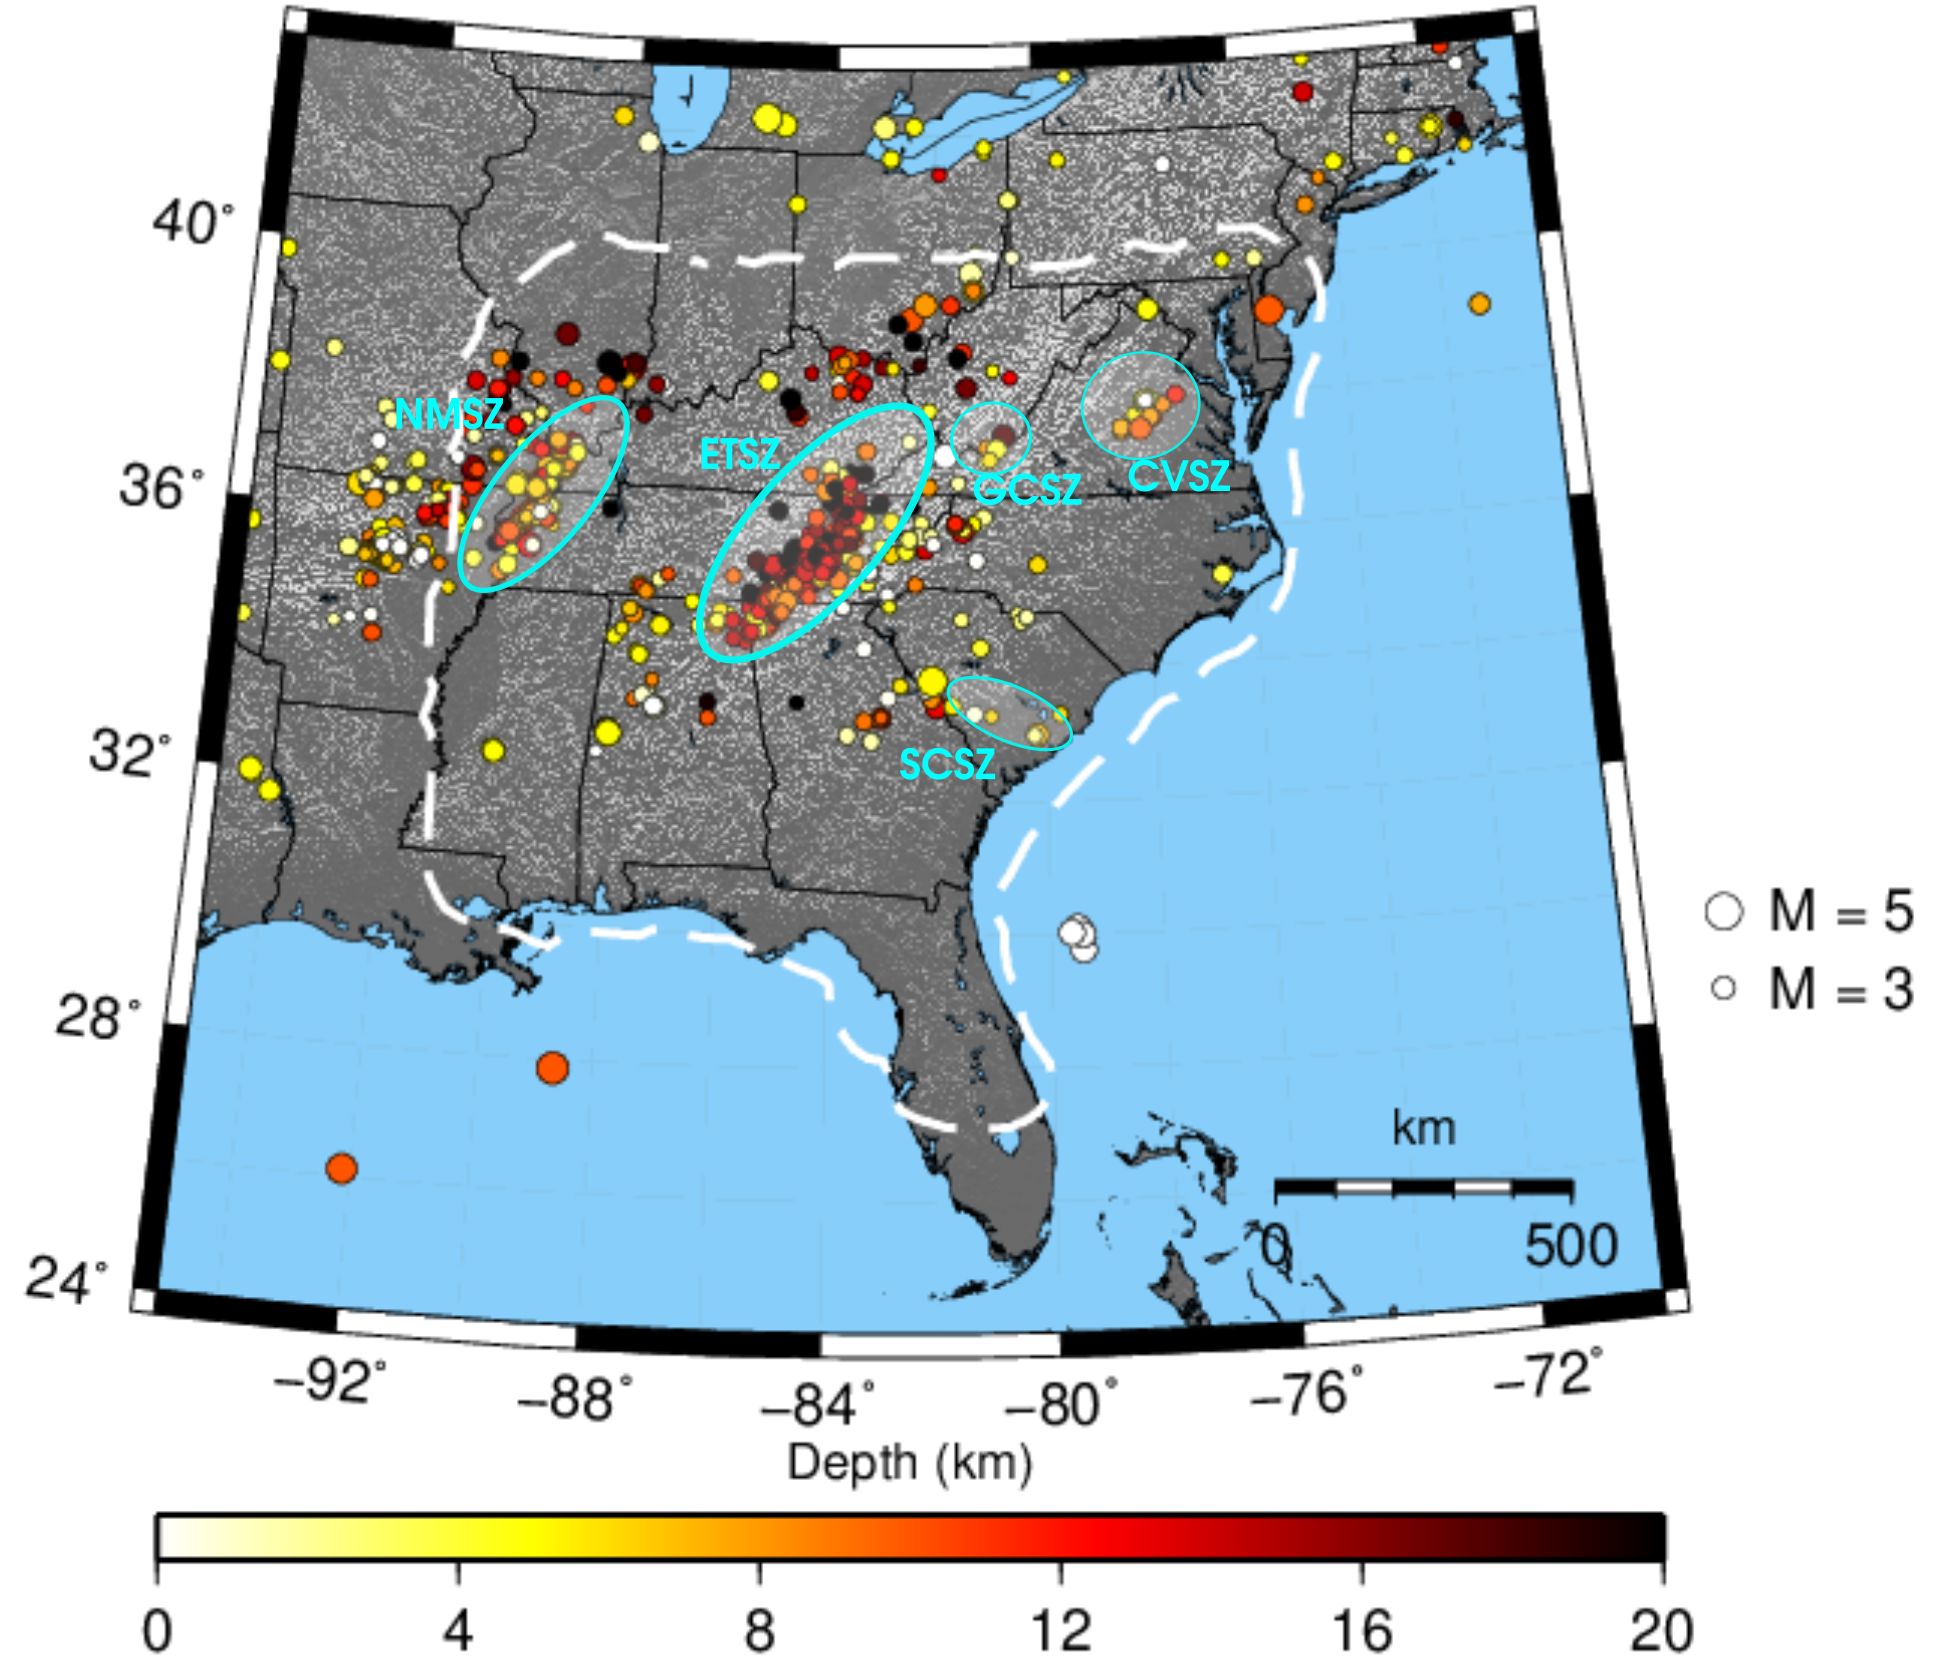
\includegraphics[width=32pc]{figures/seismicity_new.png}
    \caption{ A shaded relief map of the study area including the central and southeastern US seismic zones: New Madrid Seismic Zone (NMSZ), eastern Tennessee  Seismic Zone (ETSZ) South Carolina Seismic Zone (SCSZ), Giles County Seismic Zone (GCSZ) and Central Virginia Seismic Zone (CVSZ). White dashed line represents the well-sampled region in the tomography results by~\citet{Biryol_2016} at a depth 130 km. The earthquakes that occurred over the period December 2011 - December 2018 and had $M_{w} > 2.5$ are plotted as colored circles. The size and color of a circle represent the event's magnitude and depth. The earthquake catalog is obtained from the United States Geological Survey at \url{https://earthquake.usgs.gov/earthquakes/search/}.}
    \label{figone}
 \end{figure}
    
    Far from the tectonic plate boundaries and known to have low tectonic strain rates~\citep{Boyd_2015}, the CEUS appears to require local stress contributions to earthquake generation in the active seismic zones. Diverse origins of these local stress perturbations have been proposed, many of which involve both crustal and upper mantle heterogeneity. \citet{Kenner_2000a} proposed the presence of a weaker lower crustal zone within an elastic lithosphere that acts as a local source of stress concentration. \citet{Pollitz_2001} suggested a geodynamic model for the NMSZ consisting of a sinking mafic body in the weakened lower crust that can transfer stress into the overlying elastic crust. \citet{levandowski2016dense} showed that stress produced by a high density lower crust below the NMSZ interferes constructively with the far-field tectonic stress causing optimal stress orientations for earthquake generation.  Although the seismogenic depths in the CEUS occur in the upper to middle crust (5 to 30 km) \citep{vlahovic1998et1d, johnston1996seismic, mazzotti2010state}, deeper mantle structures can also make a significant contribution to the stress generation of  earthquakes~\citep[e.g.,][]{forte2007descent, li2007stress, chen2014crust, nyamwandha2016joint, zhan2016stress}. \citet{forte2007descent} showed that stress concentration below the NMSZ could be produced by the descent of the Farallon slab using a global geodynamic and seismic tomography based numerical model. \citet{li2007stress} showed that lateral heterogeneity in the lithosphere below the CEUS could concentrate stress. \citet{chen2014crust} and \citet{nyamwandha2016joint} independently observed a low P-wave velocity zone at 50-200 km depths below the NMSZ. This was interpreted as a weak zone which acts as a conduit for stress transfer into the crust. Similarly, based on a regional tomography model by~\citet{pollitz2014seismic}, \citet{zhan2016stress} found that weak upper mantle can focus stress in the NMSZ crust.
    
    % , with special attention given to the heterogeneities beneath the NMSZ.

    %

 %
   
%Several past studies focusing on the NMSZ have suggested that the crustal structure of this seismic zone causes stress concentration~\citep{Kenner_2000a, Pollitz_2001, levandowski2016dense}. \citet{Kenner_2000a} proposed the presence of a weaker lower crustal zone within an elastic lithosphere that acts as a local source of stress concentration. \citet{Pollitz_2001} suggested a geodynamic model for NMSZ consisting of a sinking mafic body in the weakened lower crust that can transfer stress into the overlying elastic crust. \citet{levandowski2016dense} showed that a high density lower crust below the NMSZ interferes constructively with the far-field tectonic stress causing optimal stress orientations for earthquake generation.
    
Similar considerations of crustal and mantle stress sources are yet to be made for other CEUS seismic zones such as the ETSZ, SCSZ, GCSZ, and CVSZ. In a recent high-resolution P-wave tomography study, \citet{Biryol_2016} found positive velocity anomalies in the upper mantle beneath the area in-between the ETSZ and the NMSZ at depths of 200 to 660 km, and interpreted them as foundering lithosphere. They further speculated that, since the NMSZ and ETSZ coincide with the boundary of lithosphere thinned by the drip, they are weakened by the underlying hot asthenosphere and thus prone to seismicity. 

In this study, we investigate the effects of the upper mantle heterogeneities found in the P-wave tomography study by~\citet{Biryol_2016} on the seismicity in the CEUS. We compute stress fields arising from density and strength variations converted from the tomography using instantaneous three-dimensional (3D) mantle flow models. %explaining the location of seismic zones and assessing the sources of their initiation \citep{zoback1992stress, king1994static, stein1999role, bowman2001accelerating}. 
Following previous studies that have demonstrated correlation between differential stress~\citep[e.g.,][]{baird2010relationship, zhan2016stress}) or deviatoric stresses~\citep[e.g.,][]{levandowski2016dense}) with the observed intraplate seismicity, 
% These stress indicators are useful for  observing the stress distribution within the brittle crust. 
we will consider contributions of the upper mantle heterogeneity to these stress fields and discuss the slip tendency of faults in the seismic zones based on the Coulomb failure criterion~\citep[e.g.,][]{king1994static, freed2005earthquake, li2007stress}. 


\section{Seismic tomography and upper mantle heterogeneities}
%\note[EC]{I understand your concern from your experience with the first paper but these descriptions really looks like we are doing homework for Byriol et al. They are probably useful when you present this study somewhere. Any way, let's focus on describing what was imaged.}
We briefly summarize the seismic tomography results by \citet{Biryol_2016} including the associated resolution and uncertainties before explaining our numerical models and results. The tomography study by \citet{Biryol_2016} is based on direct P and PKPdf residual travel times for the IASP91 earth model \citep{kennett1991traveltimes}. The data are collected from 514 stations in the study region (Fig. \ref{figone}) for 753 teleseismic earthquakes occurring between 2011 to 2015 with moment magnitude, $Mw > 5.5$. The discretized model has a lateral extent of 30 km in the center and 45 km along the boundary of the domain. The depth extent of the grid is from 36 km to 915 km and consists of 21 layers, but we are only interested in the features extending down to 660 km for this study. The tomographic inversion algorithm by \citet{schmandt2010seismic} is used along with optimal smoothing and damping constraints to minimize the model norm and data misfit (described in detail in the supplementary information by \citet{Biryol_2016}). Only model nodes with high quality (hit points) are used, and therefore, only model results deeper than 60 km depth are interpreted by them.
    
    \citet{Biryol_2016} verify their inversion results after robust resolution tests. The checkerboard and synthetic anomaly recovery tests indicate vertical smearing at shallow depths due to the near vertical incidence of the teleseismic raypaths and amplitude loss by about 40 \% in the center of the model. Their calculated lateral resolution in the center is about 40 km going to 60 km towards the bottom of the domain while the vertical resolution  is around 50 km at the top and increases to 65 km at the bottom. They observe some artifacts due to smearing but have overall confidence on the large magnitude ($>$1 \%) and dimensional features. The locations of the smaller dimensional features ($\sim$100 km) are recovered in the synthetic resolution tests, but their outline is smeared laterally and vertically. 
    
    The well-sampled region in the tomographic inversion shows
    %after synthetic tests 
    high-velocity anomalies with a mean amplitude of 1.9 \%, which are interpreted as lithospheric foundering (Fig.~\ref{fig_tomo}). The two perpendicular cross-sections in Fig.~\ref{fig_tomo} show that these anomalies start at about 200 km depth with lateral dimensions of $2^\circ$ and extend to 660 km where they widen to about $3^\circ$ (marked in Fig.~\ref{fig_tomo}A). According to the synthetic anomaly tests, the supposed foundering lithospheric drip with these amplitudes and dimensions should be reliably resolved.
    % and therefore, reliable for our numerical model inputs. 
%
\begin{figure}[ht]
    \centering
    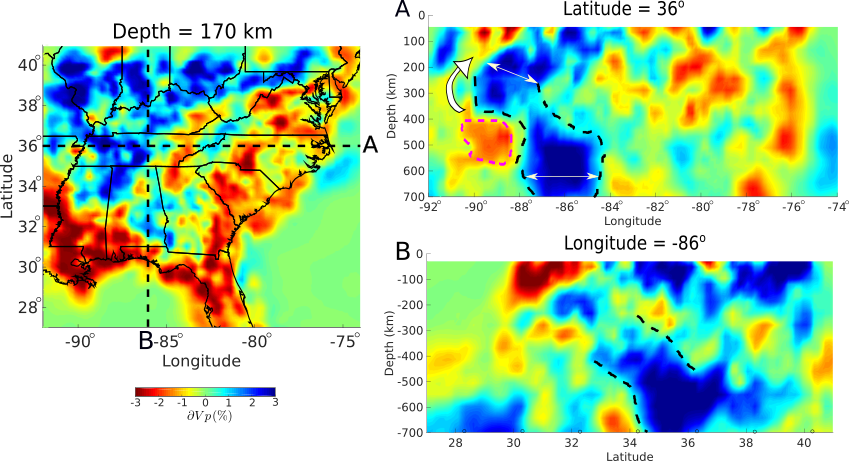
\includegraphics[width=\linewidth]{figures/figure_tomography.png}
    \caption{P wave tomography results from~\citep{Biryol_2016} at depth of 170 km. Panels A and B are cross-sections at 36$^\circ$ latitude and $-$86$^{\circ}$ longitude, respectively. Dashed black lines on the cross-sections mark the approximate boundaries of the high-density anomalies interpreted as foundering lithospheric root. Dashed magenta lines on A indicates the low-velocity region interpreted by~\citet{Biryol_2016} as asthenospheric return flow due to the foundering lithosphere. The white arrow on A shows the direction of the return flow as speculated by~\citet{Biryol_2016}.}
    \label{fig_tomo}
 \end{figure}

\section{Modeling instantaneous mantle flow}
%    Inputs for our mantle flow models include temperature and density fields converted from the velocity anomalies. The velocity-to-temperature conversion method we adopt~\citet{Cammarano2003} takes into account the effects of anelasticity, compositional variations, and phase changes. An effective power-law rheology is assumed to be \annote[EC]{a combination} of diffusion and dislocation creep. 
%To facilitate interpretation of the effects of high-density anomalies found in the upper mantle, we choose a reference model in which temperature \annote[EC]{below the model}{What does this mean?} is laterally homogeneous \note[EC]{What about radially?}. Models based on the tomography are compared with the reference model in terms of differential stress and Coulomb stress changes. The latter is computed for selected values of near-surface fault strike and dip. We also examine dynamic topography caused by the mantle flow induced by the sinking denser material.
    
\subsection{Temperature Calculations} \label{temp_var}
    Inferring temperature from the seismic velocity anomalies has the prime importance for our modeling approach because it will determine both the driving buoyancy force and the viscous resistance. We follow \citet{Cammarano2003}'s approach to calculating temperatures from the seismic velocity anomalies. This approach takes into account the effects of anharmonicity (i.e. elasticity), anelasticity and the phase transition at 410 km depth. inversion of seismic tomography results to a temperature field is commonly regarded as a non-linear problem due to the shear anelasticity of seismic waves \citep{minster1981model, karato1993importance, sobolev1996upper, Goes_2000, artemieva2004shear} and non-linear sensitivity of elastic moduli and their pressure derivatives to temperature \citep{duffy1989seismic, anderson1992high, Cammarano2003, stixrude2005thermodynamics}. The presence of melt or water may also introduce non-linearity in temperature effects on seismic velocities~\citep{Karato_1998} but the effects of melt and fluids are not considered in this study because of the lack of high heat flow and other substantial evidence for melting in this region's mantle~\citep{blackwell2006assessment}. Our inversion procedure is fully detailed in Appendix A.
%
%Both anharmonic and anelastic effects on seismic velocities \remove[EC]{, which are discontinuous at the 410 km phase transition,} are taken into account in our inversion for temperature.\note[EC]{The previous sentence is redundant with the intro paragraph of this section. Probably you don't need it.} 
    
Velocity anomalies and the inverted temperatures for depths of 200 km and 605 km are shown in Fig.~\ref{fig_temp}. 
%The temperature variations from the reference geotherm calculated from the P-wave velocity anomalies implies 
P-wave velocity (Vp) sensitivity to temperature is found to be $-$0.85 \% per 100$^\circ$K and $-$0.55 \% per 100$^\circ$K at depths 200 km and 605 km, respectively. These values are consistent with those in~\citep{Cammarano2003}: $-$0.75$\pm$0.15 \% per 100$^\circ$K and $-$0.65 \% per 100$^\circ$K at the same depths, along the mantle adiabats 1300$^{\circ}$C and 1600$^{\circ}$C, respectively, used in this study.
%
\begin{figure}[ht]
    \centering
    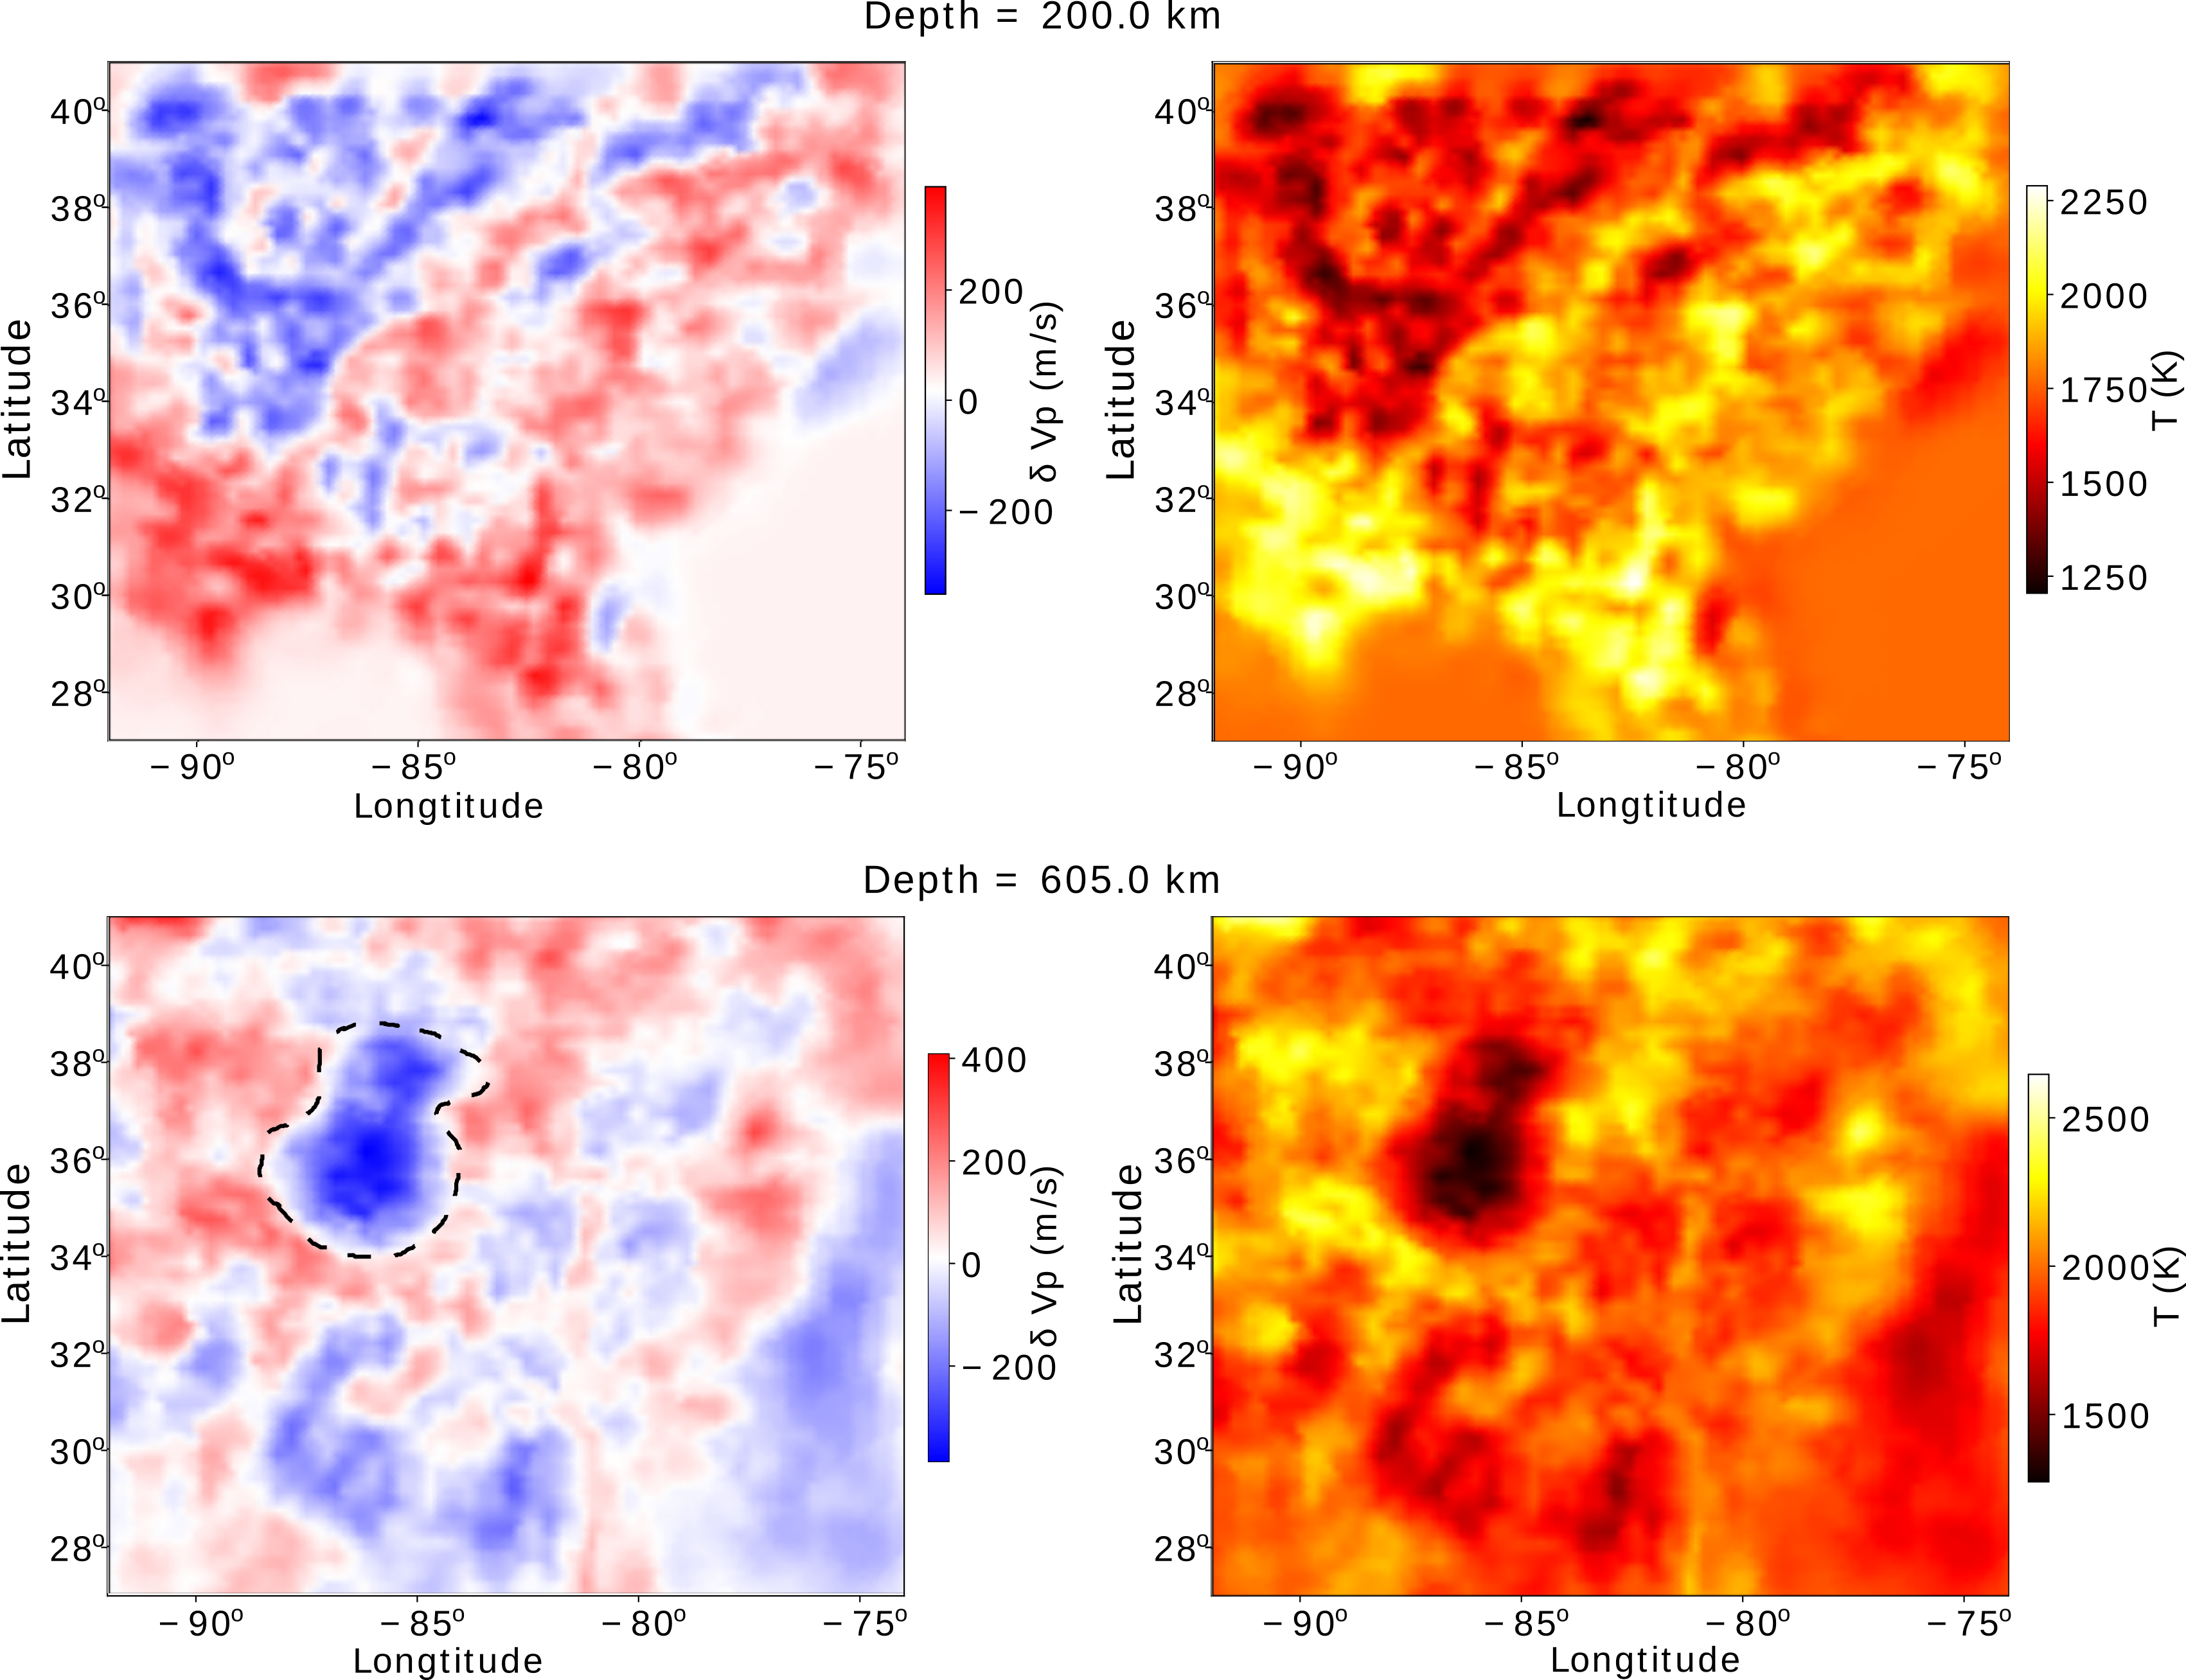
\includegraphics[width=0.75\linewidth]{figures/figure_temp.png}
    \caption{P wave anomalies (left) from~\citet{Biryol_2016} and the inverted temperatures (right) 
%    accounting for compositional variations, attenuation and the phase transformation at 410 km 
    at depths of 200 (top) and 605 km (bottom). Magenta dotted line in the depth layer 605 km marks the boundary of the high-velocity structure interpreted as a foundering drip by~\citet{Biryol_2016}.
    %, see Fig. \ref{fig_model} for a detailed structure outline.
    }
    \label{fig_temp}
 \end{figure}

\subsection{Model Setup}
  %  \note[EC]{Although a nice summary, this paragraph seems redundant and doesn't fit in the Model Setup section.} We calculate the stress field associated with an instantaneous viscous mantle flow. The mantle flow is driven by thermal buoyancy arising from the heterogeneous temperature distribution converted from the P-wave tomography by \citet{Biryol_2016} as described above. Model inputs, density, and viscosity distributions are computed based on the converted temperatures. 
    
    We compute velocity and stress fields that are in equilibrium with heterogeneous buoyancy forces arising from the heterogeneous distribution of temperature-dependent density. For this calculation, we use an open-source finite element code, ASPECT version 2.0.0~\citep{heister_aspect_methods2,KHB12,aspect-doi-v2.0.0}. ASPECT can solve the equations for the conservation of mass, momentum, and energy using an adaptive finite element method for a variety of rock rheologies. 
    
     Our model domain is laterally bounded by longitudes, 71$^{\circ}$W and 95.5$^{\circ}$W and by latitudes, 23$^{\circ}$N and 43$^{\circ}$N. The depth range is from 0 to 660 km (Fig.~\ref{fig_model}). Since the tomography model considers only the mantle starting from a depth of 36 km, we assume \annote[EC]{a laterally homogeneous crust with 4 depth layers such that the temperature and density increase linearly with depth.}{This is confusing. Do you mean the 36 km-thick crust is divided into 4 layers or the crust is one of the 4 layers? Also it would be better to plot and show the temperature and density increase with depth.}  %In the crust, composition, physical conditions and material properties are assumed to be laterally homogeneous such that temperatures and density, and viscosity are 500 $^{\circ}$C, 2900 kg/m$^{3}$, and 5x10$^{24}$Pa$\cdot$s, respectively.
%Our interest only in heterogeneous mantle stress sources justifies this assumption of a homogeneous crust. 
The domain is discretized into 0.512 million hexahedral elements with a 0.15$^{\circ}$ resolution in longitude, 0.125$^{\circ}$ in latitude and 35 km in depth. This spatial resolution is similar to that of the tomography and thus sufficient for resolving the mantle structures shown by the tomography model. 

We assessed mesh resolution effects by running a model with a twice finer mesh having 2.048 million elements and found that differences in the results were small: relative error of 2\% in the velocity field. All the model results presented in this study are thus based on the coarse mesh for computational efficiency. We also tested a model with an additional lateral area of 5$^{\circ}$ by 5$^{\circ}$ surrounding our domain to asses boundary effects. The overall resultant velocity and stress field are similar with those for the smaller model domain, but the magnitude of the calculated stress and velocity field at our depth of interest, i.e. 15 km, near the boundaries is smaller by 10-15 \% because the viscous effect of the same heterogeneity is now spread over a larger area. However, since the seismic zones are sufficiently far from the model domain boundaries, we show only the results for the smaller domain.
%
\begin{figure}[ht]
    \centering
    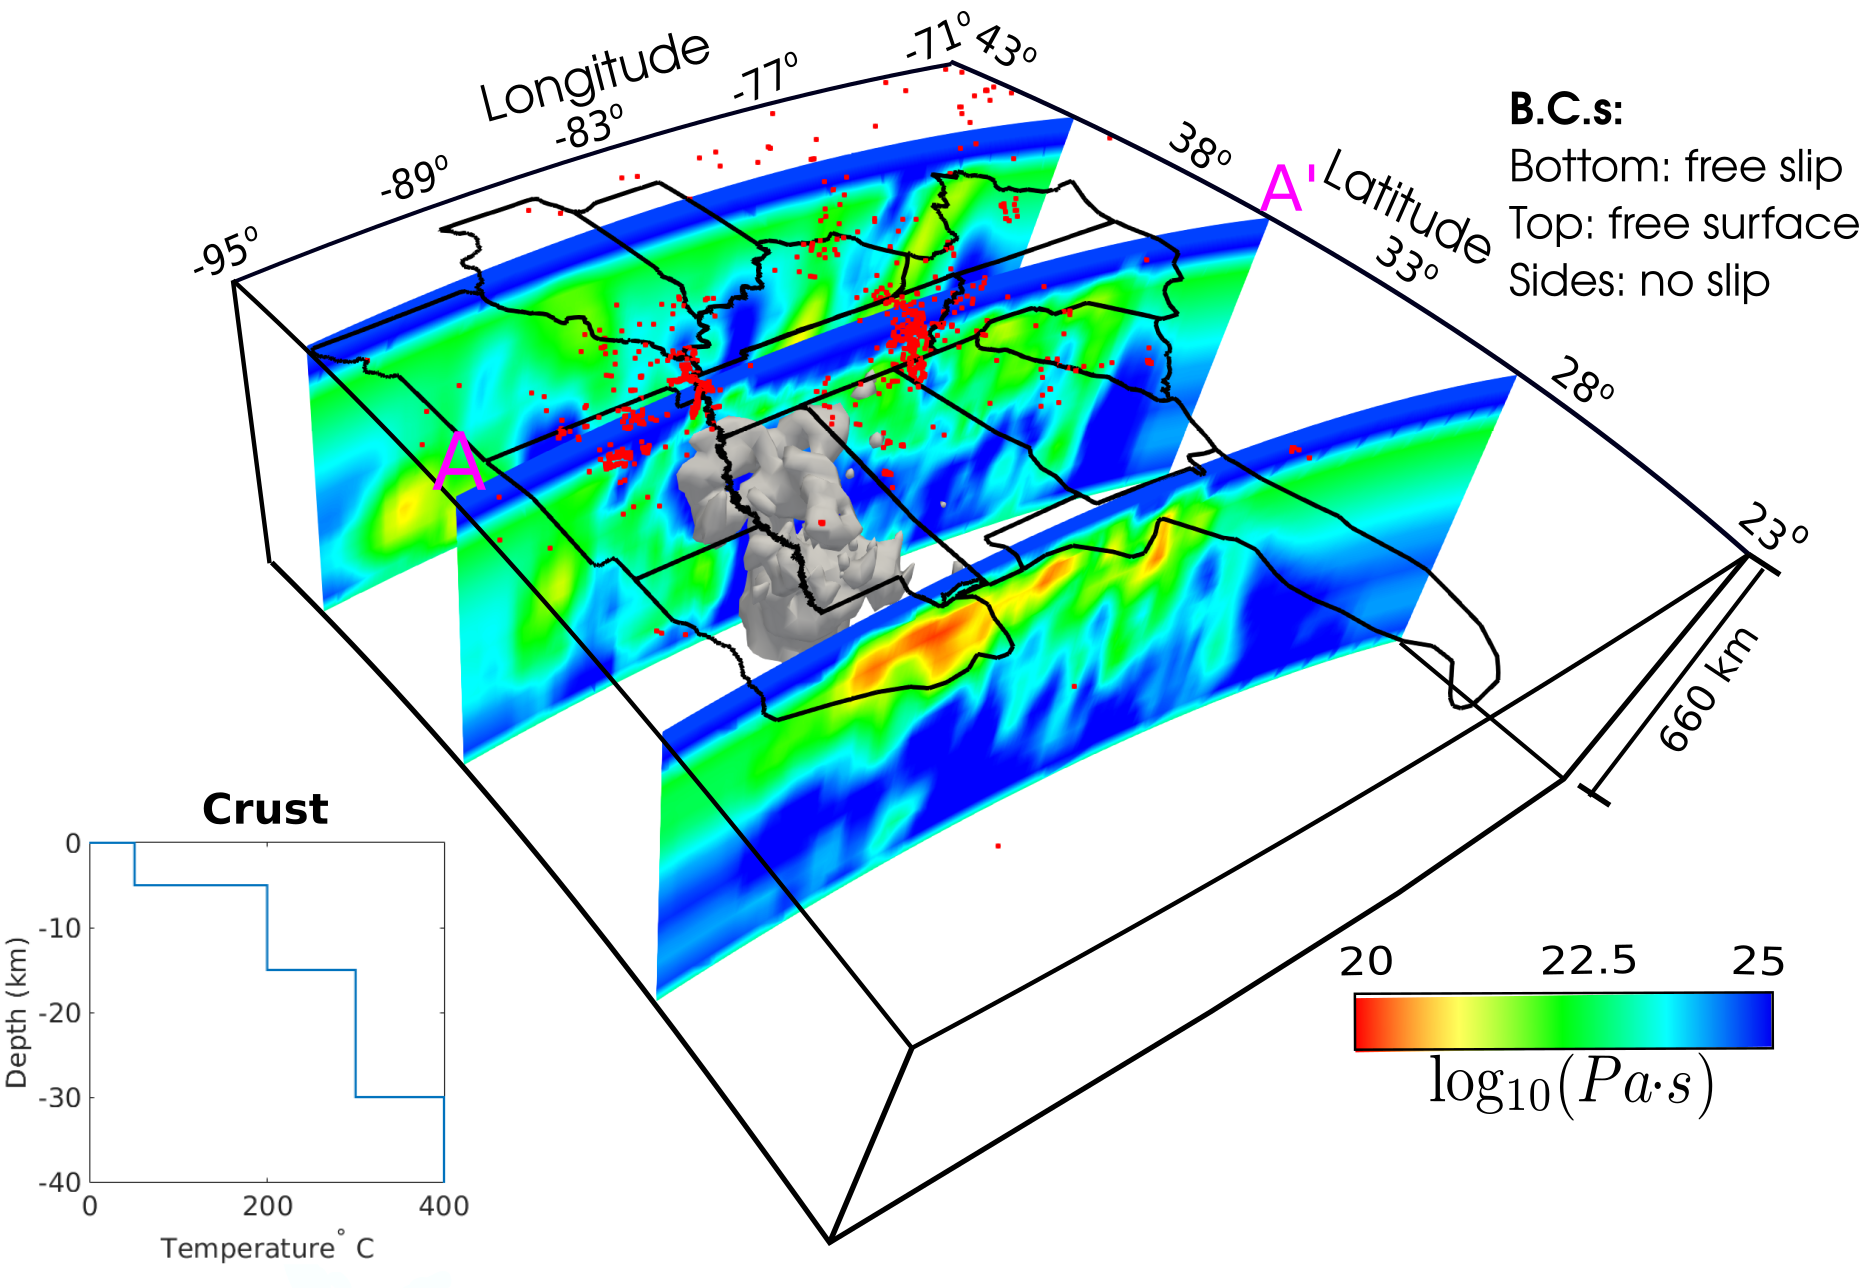
\includegraphics[width=0.75\linewidth]{figures/model_figure.png}
    \caption{Model setup with the computed rheology based on the regional tomography by \citet{Biryol_2016} and the boundary conditions applied. Gray isosurface represents P-wave anomalies $>$ 2 \% in the region interpreted as lithospheric foundering. Instantaneous flow along slice AA' passing through the ETSZ and NMSZ is discussed in Fig. \ref{velocity_pattern}. Black lines indicate the state boundaries and red dots are the epicenters for the earthquake catalog used in Fig. \ref{figone}}.
    \label{fig_model}
\end{figure}

Upper mantle flow is assumed to occur by a dislocation creep at low temperatures relative to the melting temperatures of mantle rocks and by a diffusion creep at higher temperatures~\citep[e.g.,][]{gordon1967thermally}. Our model employs both dislocation and diffusion creep with each type having different contributions depending on the temperature and pressure. In this rheology model, the effective viscosity ($\eta_{\text{eff}}$) is computed as~\citep{billen2007rheologic}:
%
\begin{align}
    \eta_{\text{i}} &= \frac{1}{2} A^{-\frac{1}{n_i}} d^\frac{m_i}{n_i} \dot{\varepsilon_i}^{\frac{1-n_i}{n_i}} \exp\left(\frac{E_i + PV_i}{n_iRT}\right),\ i=\text{diff or dis}, \\
    \eta_{\text{eff}} &= \left(\frac{1}{\eta^\text{diff}} + \frac{1}{\eta^\text{dis}}\right)^{-1},
\end{align}
%
where diff and dis denote diffusion and dislocation creep, $A_i$ is the pre-exponential factor, $n_i$ is the power law exponent, $d$ is the grain size, $m_i$ is the grain size exponent, $\dot{\varepsilon}$ is the second invariant of the strain rate tensor, $R$ is the gas constant, $T$ is temperature obtained from the inversion of the Vp anomalies, $P$ is pressure, and $E_i$ and $V_i$ are the activation energy and volume, respectively. All the parameter values used in this study are given in Table~\ref{table_model}.
%
\begin{table}[ht] 
    \caption{Values for dislocation and diffusion creep}
    \centering
    \begin{tabular}{l c c c c}
    \hline
     Parameter  & Symbol & Unit & Diffusion Creep & Dislocation Creep  \\
    \hline
      Pre-exponential factor$^a$ & $A$ & $s^{-1}$ & 1.5 $\times$ 10$^{-16}$ & 0.3 $\times$ 10$^{-22}$   \\
      Power law exponent$^a$ & $n$ & & 1 & 3.5  \\
      Grain size exponent$^a$  & $m$ & & 2 & 0   \\
      Activation energy$^a$  & $E$ & kJ/mol & 300 & 530   \\
      Activation volume$^a$  & $V$ & cm$^3$/mol & 6 & 20 \\
      grain size$^b$         & $d$ & mm & 5 & 5 \\
    \hline
    \multicolumn{5}{l}{$^{a}$\citet{karato1993rheology}. $^b$Approximate value for olivine~\citep{karato1984grain}.}
    \end{tabular}
    \label{table_model}
\end{table}

The bottom boundary at 660 km has the free-slip condition~\citep[e.g.,][]{arcay2007slab, billen2007rheologic, quinquis2011role}. For side boundaries, we tested our model with both free-slip and no-slip conditions and verified that the velocity fields at the seismic zones have the same pattern with up to 5\% magnitude difference. In this study, we only show the results for the no-slip conditions. We let the top boundary be a free surface that can develop topography in response to the instantaneous flow in the mantle. 
%I don't think you need explain this: based on \citet{kaus2010stabilization} free surface stabilization implemented in ASPECT) 

\subsection{Differential and Coulomb stress changes}
We define static changes in Coulomb stress ($\Delta C$) of a model with respect to another model as the difference in Coulomb Failure Function (CFF)~\citep{king1994static}:
%
\begin{equation}
    \Delta C = \Delta \tau - \mu' \Delta \sigma_n,
\end{equation}
%
where $\Delta \tau$ and $\Delta\sigma_n$ are the difference between the models in shear (positive in the direction of slip) and normal (positive when compressive) stress for a particular fault orientation, and $\mu'$ is the effective coefficient of friction after accounting for pore pressure. Since we do not have sufficient constraints on the effective friction coefficients for the faults in the study area, we use a value of 0.6 based on the study by~\citet{hurd2012intraplate}. Differential stress, $\sigma_{\text{diff}} \equiv \sigma_{1}-\sigma_{3}$, are compared between different models with a similarly defined quantity, $\Delta \sigma_{\text{diff}}$.

Stress tensors in the model outputs are given as Cartesian stress components with respect to $x$ and $y$ axes at 0$^{\circ}$ and 90$^{\circ}$ longitudes and on the equator. Stress tensors are transformed according to a rotation of the model domain by which the $z$ axis goes through the center of the domain. After this rotation, $x$ and $y$ axes approximately coincide with East and North as understood in the model. Stress tensors are further transformed such that $x$, $y$ and $z$ axes in the rotated Cartesian system coincide with a fault\rq{}s strike, up-dip and normal directions (Fig.~\ref{signs}). We follow the convention that strike is defined as the direction that puts a dipping fault plane on the right and dip angle changes between 0$^{\circ}$ and 90$^{\circ}$. %surface  is located at the  follow the right-hand rule such that dips are measured on the right side of the footwall facing the fault strike and 
In the final coordinate system, negative values of $\tau_{zx}$ and $\tau_{zy}$ correspond to right-lateral and down-dip sense of motion, respectively.
% High $\mu$ between 0.5 and 0.8 is associated with \annote[EC]{limited}{What do you mean?} fault cohesion and therefore, \annote[EC]{slip while lower values, i.e. 0-0.5 are generally taken for smooth sealed faults capable of larger slip accumulation}{The meaning of this sentence is not clear to me.} \citep{parsons1999stress}. 
%
\begin{figure}[h!]
    \centering
    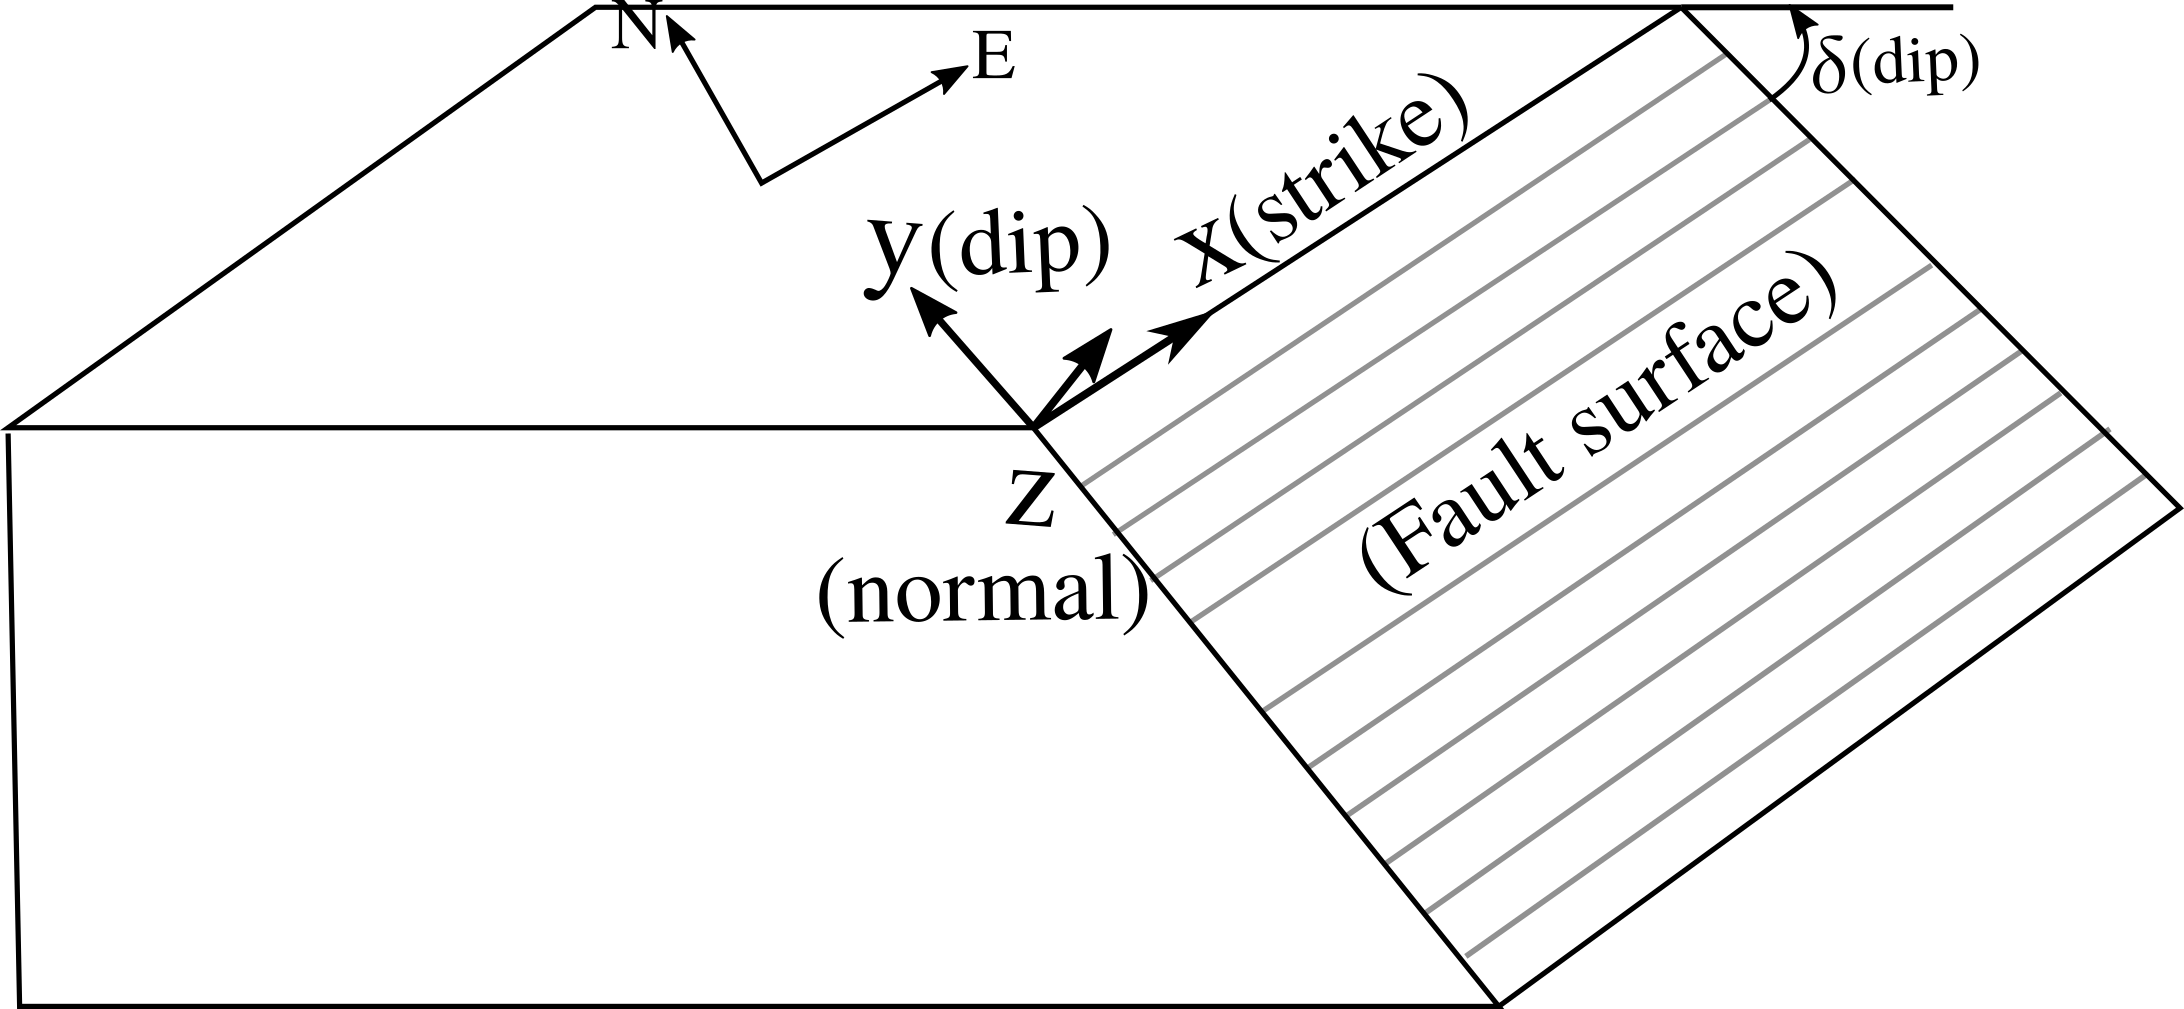
\includegraphics[width=0.5\linewidth]{figures/sign_convention.png}
    \caption{Cartoon sketch showing the sign convention for the strike, dip, and normal to the fault surface. \note[EC]{Please try to show that the x, y and z axes in the current figure are the rotated ones from the \lq\lq{}north\rq\rq{} and \lq\lq{}east\rq\rq{}. Also, $z$ axis should be re-oriented so that it can look normal to the fault plane.} }
    \label{signs}
\end{figure}

To facilitate comparison of models with and without the local upper-mantle heterogeneity, delineated by the velocity anomaly isosurface in Fig.~\ref{fig_model}, we denote the tomography-based model with the foundering lithosphere as HT (HeTerogeneous), a model with laterally homogeneous temperature in the upper mantle as HM (HoMogeneous), and a model identical with HT except that the temperature within the foundering lithosphere is replaced with the reference values as HR (Homogeneous but having the Root). Fig.~\ref{model_differences} shows a cross-section of the tomography illustrative of these model setups. HT$-$HM represents the contributions from the upper mantle heterogeneity, while HT$-$HR shows only the contribution of the high-velocity structure interpreted as the foundering drip (Fig.~\ref{model_differences}).  Coulomb stress changes, $\Delta$C$_{HT-HM}$ and $\Delta$C$_{HT-HR}$, indicates whether and how much the stress field in the model HT would promote the slip tendency of a fault relative to stress fields in HM and HR. For instance, a positive $\Delta$C$_{HT-HM}$ for a fault geometry and a sense of motion means that the mantle heterogeneities considered in HT promote the failure of the fault relative to the laterally homogeneous mantle (HM). 
%
\begin{figure}[h!]
    \centering
    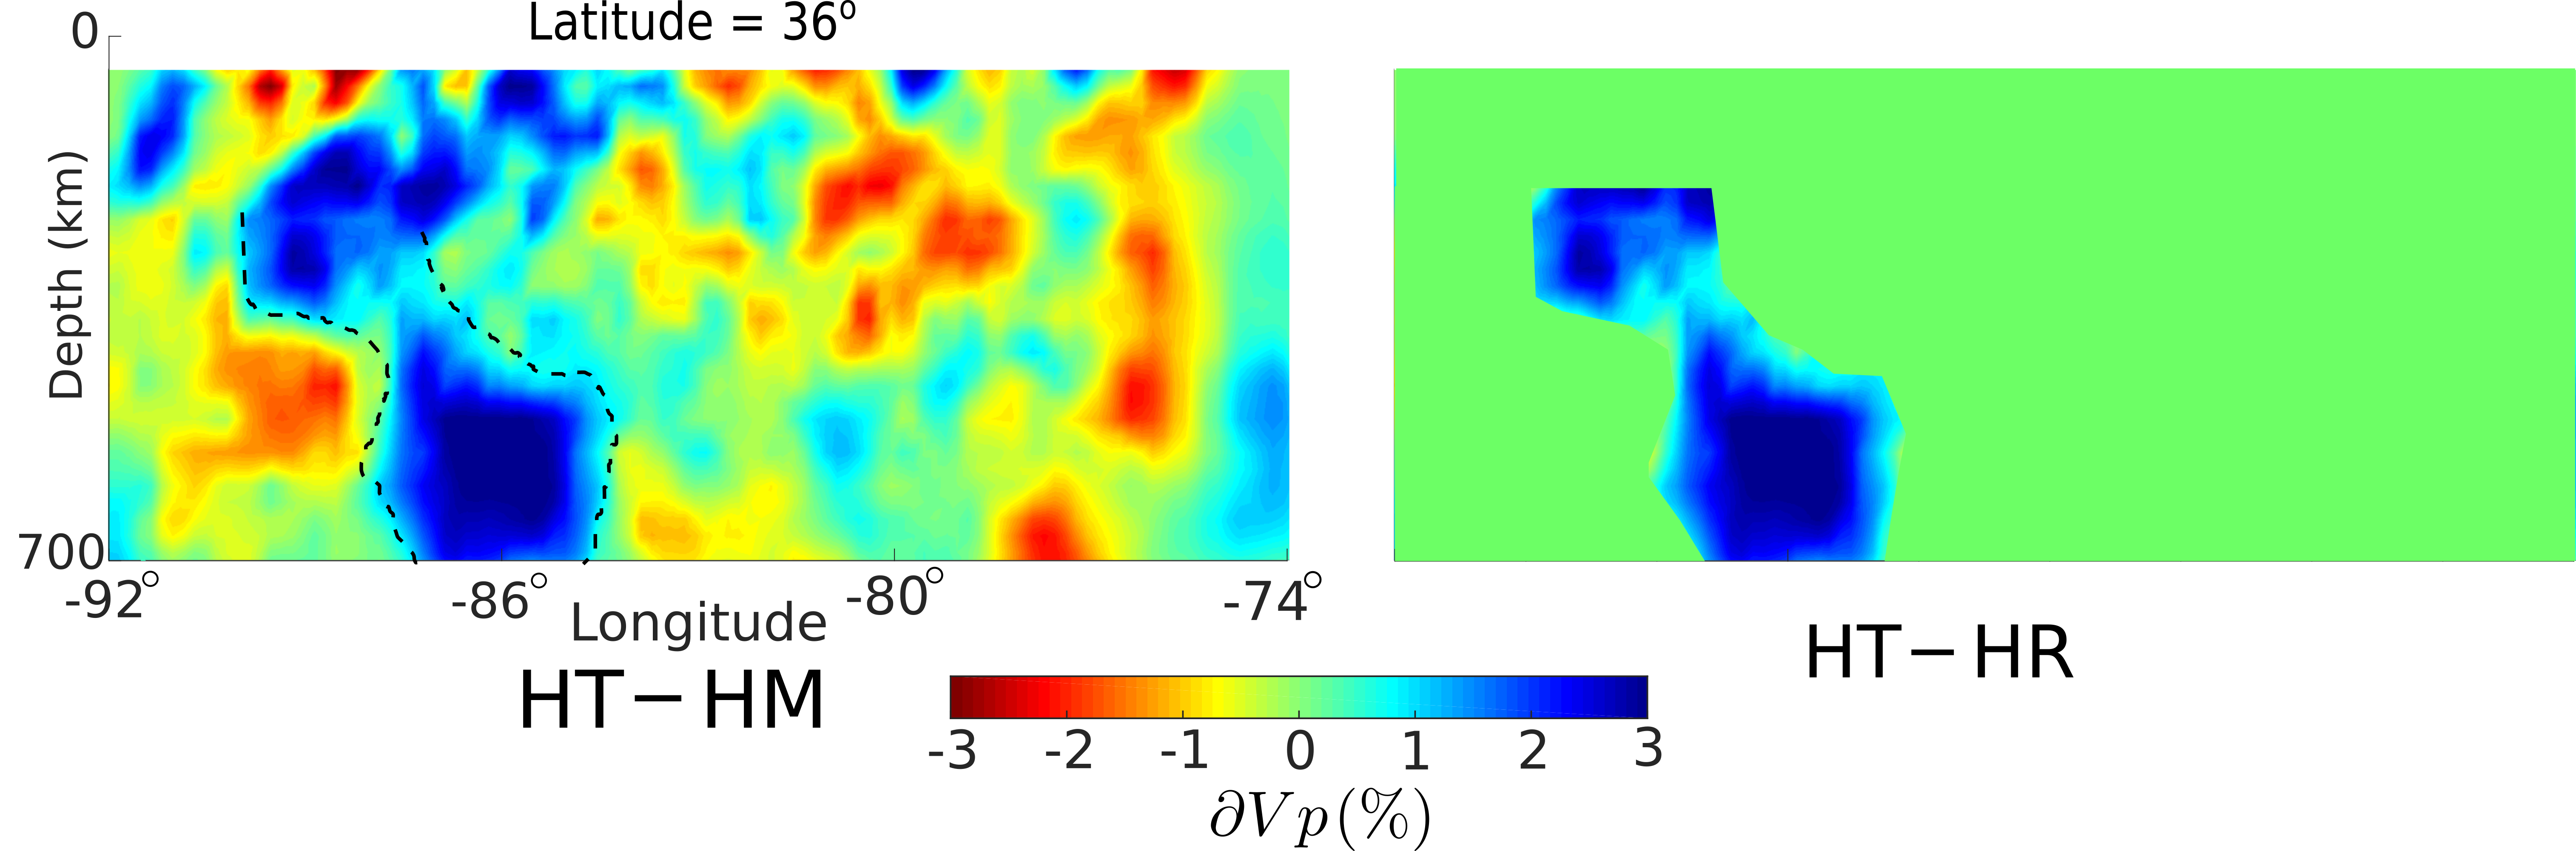
\includegraphics[width=\linewidth]{figures/model_differences.png}
    \caption{Cross-section across different model setups based on the tomography results~\citep{Biryol_2016}, and the corresponding acronym used in this study. HT (heterogeneous) accounts for all of the upper mantle seismic anomalies, HM (homogeneous) assumes laterally homogeneous upper mantle, and HR (homogeneous root) assumes no anomalies in the region interpreted as the lithospheric drip (Fig.~\ref{fig_model}). The model differences HT$-$HM and HT$-$HR are examined to observe the effects of upper mantle heterogeneity and lithospheric drip, respectively. \note[EC]{Now, HT-HM is too trivial to show. Maybe we keep only HT-HR?}}
    \label{model_differences}
\end{figure}

We calculate $\Delta C$ and $\Delta \sigma_{\text{diff}}$ for HT$-$HM and HT$-$HR, and analyze the results at the approximate locations of the seismic zones, ETSZ, SCSZ, CVSZ, GCSZ, and the northeastern arm of the NMSZ (NMSZ\_NE) (shown in Fig.~\ref{df_model}), which are contained in the well-resolved region in the~\citet{Biryol_2016} tomography. CFF values are computed for the optimal fault geometries based on the focal mechanisms and earthquake relocations at 15 km depth in all the seismic zones (Table \ref{table_fault}). 
%To quantify the correlation of seismic zones with an increased $\Delta$C, we use a slip coefficient, $\Theta$, defined as the fraction of points in a seismic zone that exceed $\Delta C = 0.5$ MPa for a particular fault orientation. We choose the threshold of 0.5 MPa based on the study by~\citet{stein1999role} which suggests that for optimally orientated faults, stress perturbation as low as 0.5 MPa can cause a fault to slip.
%
\begin{table}
\caption{Seismic Zones$^{*}$ and their associated \annote[EC]{optimal}{Is optimal an optimal term?} fault geometries}
\centering
\begin{tabular}{ l l l l } 
    \hline
    Seismic Zone & Strike, Dip & Sense of motion & Reference \\
    \hline
    NMSZ\_NE &  N$10^\circ$E, 90$^\circ$ & right-lateral & \citet{chiu1992imaging, shumway2008focal} \\ 
    \multirow{2}{2em} {ETSZ\ \ \ } & \multirow{2}{7em}{1- N$10^\circ$E, 90$^\circ$; 2- E-W, 90$^\circ$} &  \multirow{2}{6em}{right-lateral; left-lateral} &  \multirow{2}{20em} {\citet{chapman1997statistical, cooley2015new, powell2016grenville}} \\ & & & \\
    %ETSZ & N$10^\circ$E, 90$^\circ$ & right-lateral & \citet{chapman1997statistical, cooley2015new, powell2016grenville} \\
    %         & E-W, 90$^\circ$              & left-lateral    &   \\
    GCSZ & E-W, 90$^\circ$ & left-lateral  & \citet{munsey1985focal} \\ 
    CVSZ & N$30^\circ$E, 50$^\circ$SE & thrust  & \citet{wu2015aftershock}  \\ 
    SCSZ & N$180^\circ$E, 40$^\circ$W & thrust & \citet{chapman2016modern}\\    
    \hline
\end{tabular}
 \begin{tablenotes}
    \begin {small}
        \item[1] $^{*}$ NMSZ\_NE: North eastern arm of New Madrid Seismic Zone; ETSZ: Eastern Tennessee Seismic Zone; GCSZ: Giles County Seismic Zone; CVSZ: Central Virginia Seismic Zone; SCSZ: South Carolina Seismic Zone.  \note[EC]{The bibliography for Cooley 2015 should be completed.}
     \end{small}
  \end{tablenotes}
\label{table_fault}
\end{table}


%%%
\section{Model results}
%
The upper mantle heterogeneity results in increased differential stresses at crustal depths and at the CEUS seismic zones. $\Delta \sigma_{\text{diff}}^{\text{HT}-\text{HM}}$
%are computed at (i.e., $\Delta \sigma_{\text{diff,HT-HM}} = \sigma_{\text{diff,HT}}-\sigma_{\text{diff,HM}}$)
%$\Delta|\sigma_1 - \sigma_3| = |\sigma_1 - \sigma_3|_{HT} - |\sigma_1 - \sigma_3|_{HM}$)
is plotted in Fig.~\ref{df_model}a for the depth of 15 km, at which seismicity in the study area is most frequent~\citep[e.g.,][]{mazzotti2010state}. The seismic zones, ETSZ, SCSZ, GCSZ, CVSZ, and NMSZ, are correlated with positive $\Delta \sigma_{\text{diff}}^{\text{HT}-\text{HM}}$ in the range of 30 to 40 MPa (Fig.\ref{df_model}b). The areas F$_{1}$ and F$_{2}$ marked on Fig.\ref{df_model}a do not show active seismicity but $\Delta \sigma_{\text{diff}}^{\text{HT}-\text{HM}}$ is greater than 70 MPa. In contrast, $\Delta\sigma_{\text{diff}}^{\text{HT}-\text{HR}}$ shows only small positive values, 2 to 4 MPa in the horseshoe-shaped region surrounding the drip, which partially overlaps with the ETSZ and NMSZ (Fig.\ref{df_model}b).
%
\begin{figure}[h!]
    \centering
    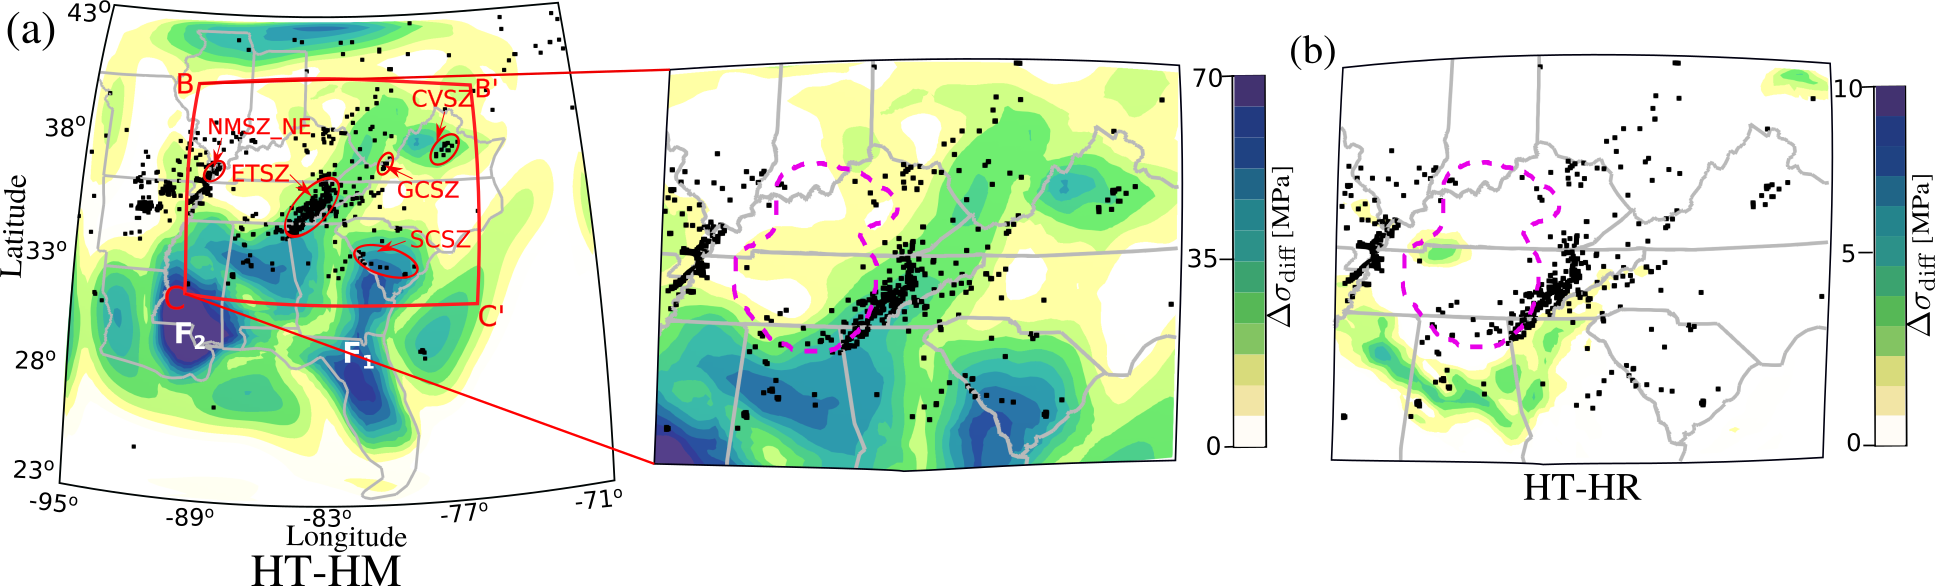
\includegraphics[width=\linewidth]{figures/diff_stress_model.png}
    \caption{(a) Differential stress changes in the HT$-$HM case ($\Delta \sigma_{\text{diff}}^{\text{HT}-\text{HM}}$) at a depth of 15 km. Black dots are earthquake epicenters from USGS data between 2011-2018. Gray lines denote the US state boundaries. Seismic zones investigated in this study are the northeastern arm of the New Madrid Seismic Zone (NMSZ\_NE), Eastern Tennessee Seismic Zone (ETSZ), South Carolina Seismic Zone (SCSZ), Giles County Seismic Zone (GCSZ) and Central Virginia Seismic Zone (CVSZ). F$_1$ and F$_2$ indicates the areas of anomalously high values of $\Delta \sigma_{\text{diff}}^{\text{HT}-\text{HM}}$. Dashed magenta line marks the boundary of the foundering at 605 km depth. The box BB'CC' indicates the region enlarged in subsequent figures. (b) Differential stress change for HT$-$HR ($\Delta \sigma_{\text{diff}}^{\text{HT}-\text{HR}}$) in a region centered on the ETSZ. }
    \label{df_model}
\end{figure}

The presence of upper mantle heterogeneity increases the Coulomb stress in  all of the seismic zones for their respective optimal fault orientations listed in Table~\ref{table_fault}. $\Delta \sigma_{\text{diff}}^{\text{HT}-\text{HM}}$, Coulomb stress changes for HT$-$HM
%along with the seismic zones and their optimal fault geometry considered (Table~\ref{table_fault}). 
%The heterogeneous HT$-$HM produces a stress field that would increase the Coulomb stress 
is about 5 MPa in the GCSZ and in the  ETSZ for their optimal fault orientations (Fig.~\ref{ht_hm_cs}a). On the other hand, $\Delta$C$_{\text{HT}-\text{HM}}$ 
for a vertical right-lateral fault striking N10$^{\circ}$E 
indicates that the mantle heterogeneities reduce the slip tendency in the ETSZ but slightly increases it in the NMSZ\_NE (Fig.~\ref{ht_hm_cs}b). 
$\Delta \sigma_{\text{diff}}^{\text{HT}-\text{HM}}$ is about 20 MPa for the thrust motion on the dominant fault orientations in the CVSZ and the SCSZ (Fig.~\ref{ht_hm_cs}c,d). 
 %, which is the  for shows not much correlation between the seismicity in SCSZ and positive $\Delta $C (Fig. \ref{model_results}(c)). 
%
\begin{figure}[h!]
    \centering
    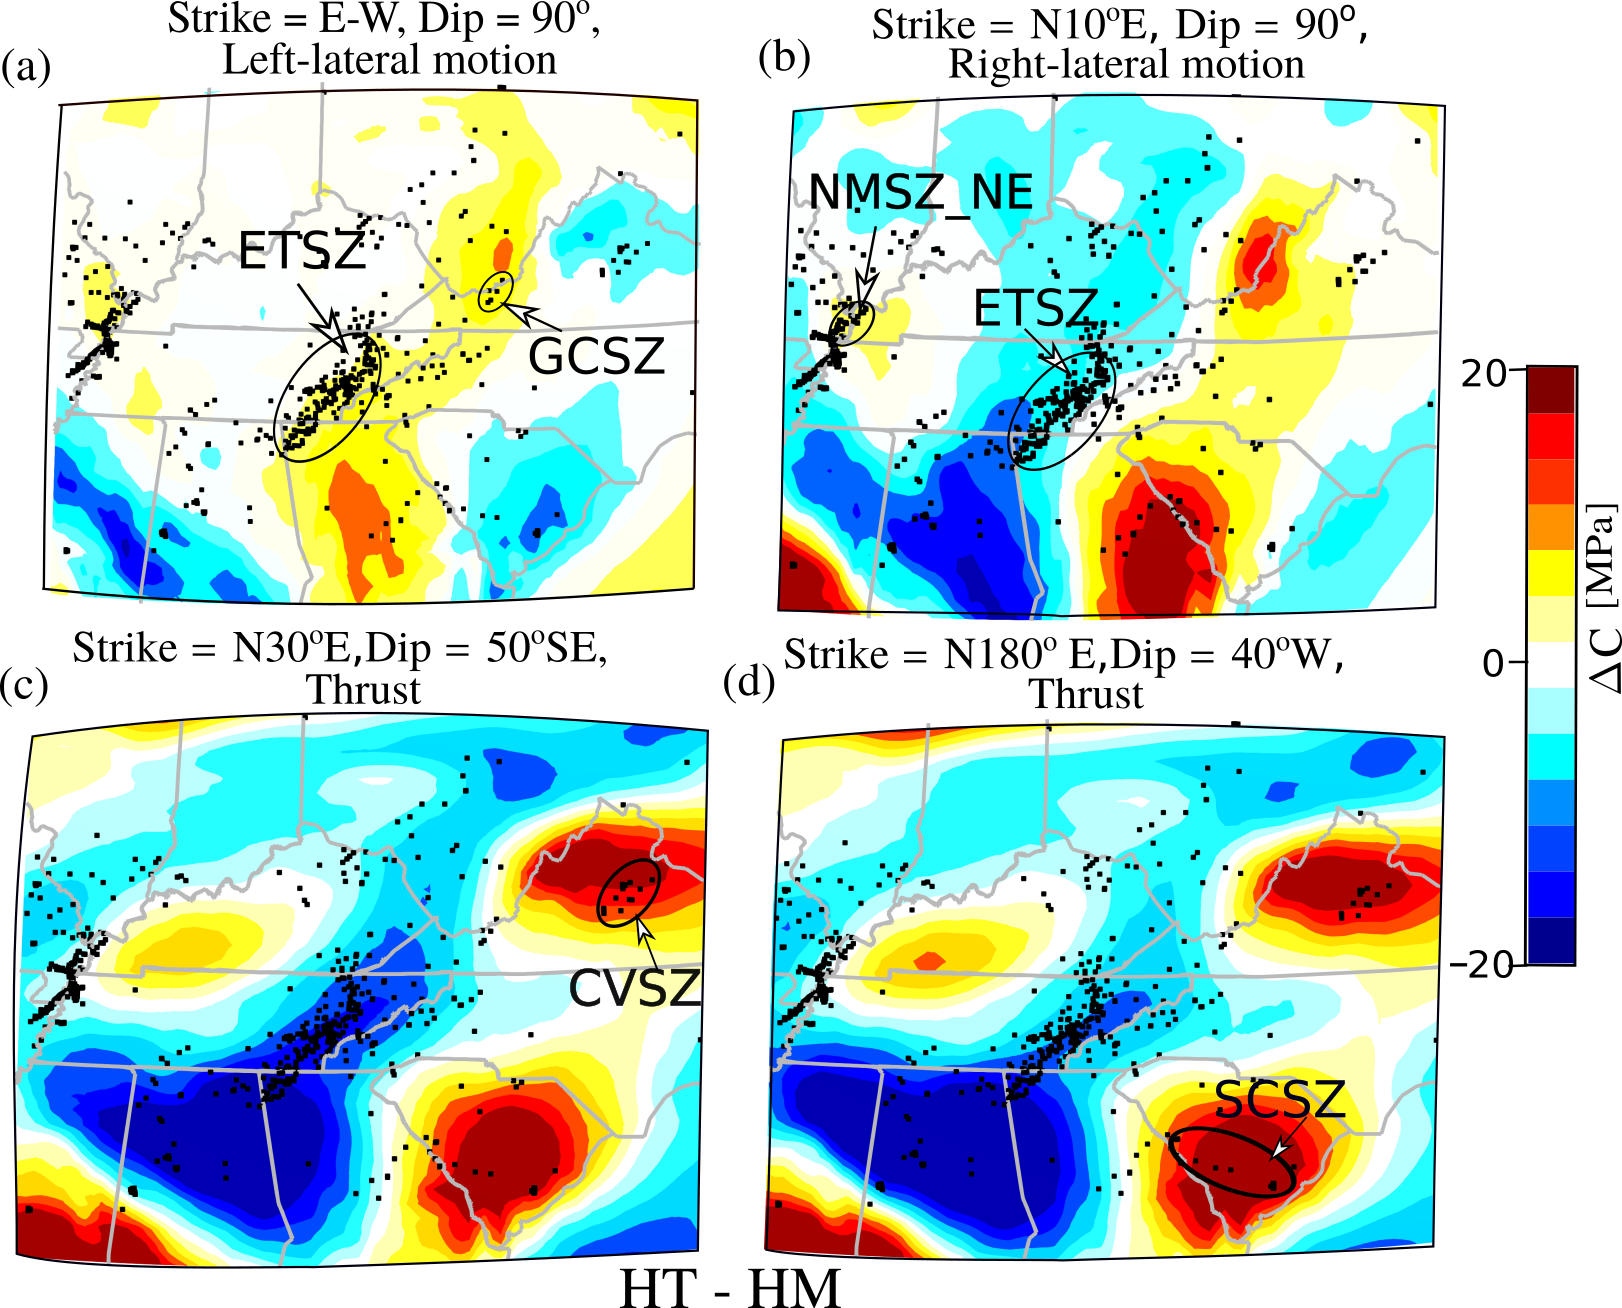
\includegraphics[width=0.75\linewidth]{figures/cs_ht_hm.png}
    \caption{Coulomb stress change ($\Delta$C) for HT$-$HM calculated for different fault orientations ({Why do you call it northern? To me, it seems to be the eastern half of the ETSZ or even possibly almost all of the ETSZ.} in Table~\ref{table1}) at 15 km depth. Seismic zone(s) and their corresponding optimal fault geometries are mentioned for each subplot: (a) Eastern Tennessee Seismic Zone (ETSZ) and Giles County Seismic Zone (GCSZ), left lateral vertical fault striking EW, (b) ETSZ and North-eastern arm of the New Madrid Seismic Zone (NMSZ\_NE) and right lateral vertical fault strikingt N10$^\circ$E, (c) Central Virginia Seismic Zone (CVSZ) and thrust fault dipping 50$^\circ$ SE striking N30$^\circ$E, (d) South Carolina Seismic Zone (SCSZ) and thrust fault dipping 40$^\circ$ W striking N-S.}	
    \label{ht_hm_cs}
\end{figure}

Coulomb stress changes due to the lithospheric drip ($\Delta$C$_{\text{HT}-\text{HR}}$) is mostly negative or weakly positive at all the seismic zones for their respective dominant fault orientations (Fig.~\ref{ht_hr_cs}). $\Delta$C$_{\text{HT}-\text{HR}}$ tends to be confined to an area surrounding the drip making relatively greater impact on the ETSZ and NMSZ than on the other seismic zones further east. $\Delta$C$_{\text{HT}-\text{HR}}$ is about 1-2 MPa in the NMSZ\_NE for its dominant fault orientations (Fig. \ref{ht_hr_cs}b) but decreases at the ETSZ for both of the dominant orientations (Fig.~\ref{ht_hr_cs}a, b). The GCSZ, CVSZ and SCSZ are located too far from the drip to have significant $\Delta$C$_{\text{HT}-\text{HR}}$ (Fig.~\ref{ht_hr_cs}a, c and d).

\begin{figure}[ht]
    \centering
    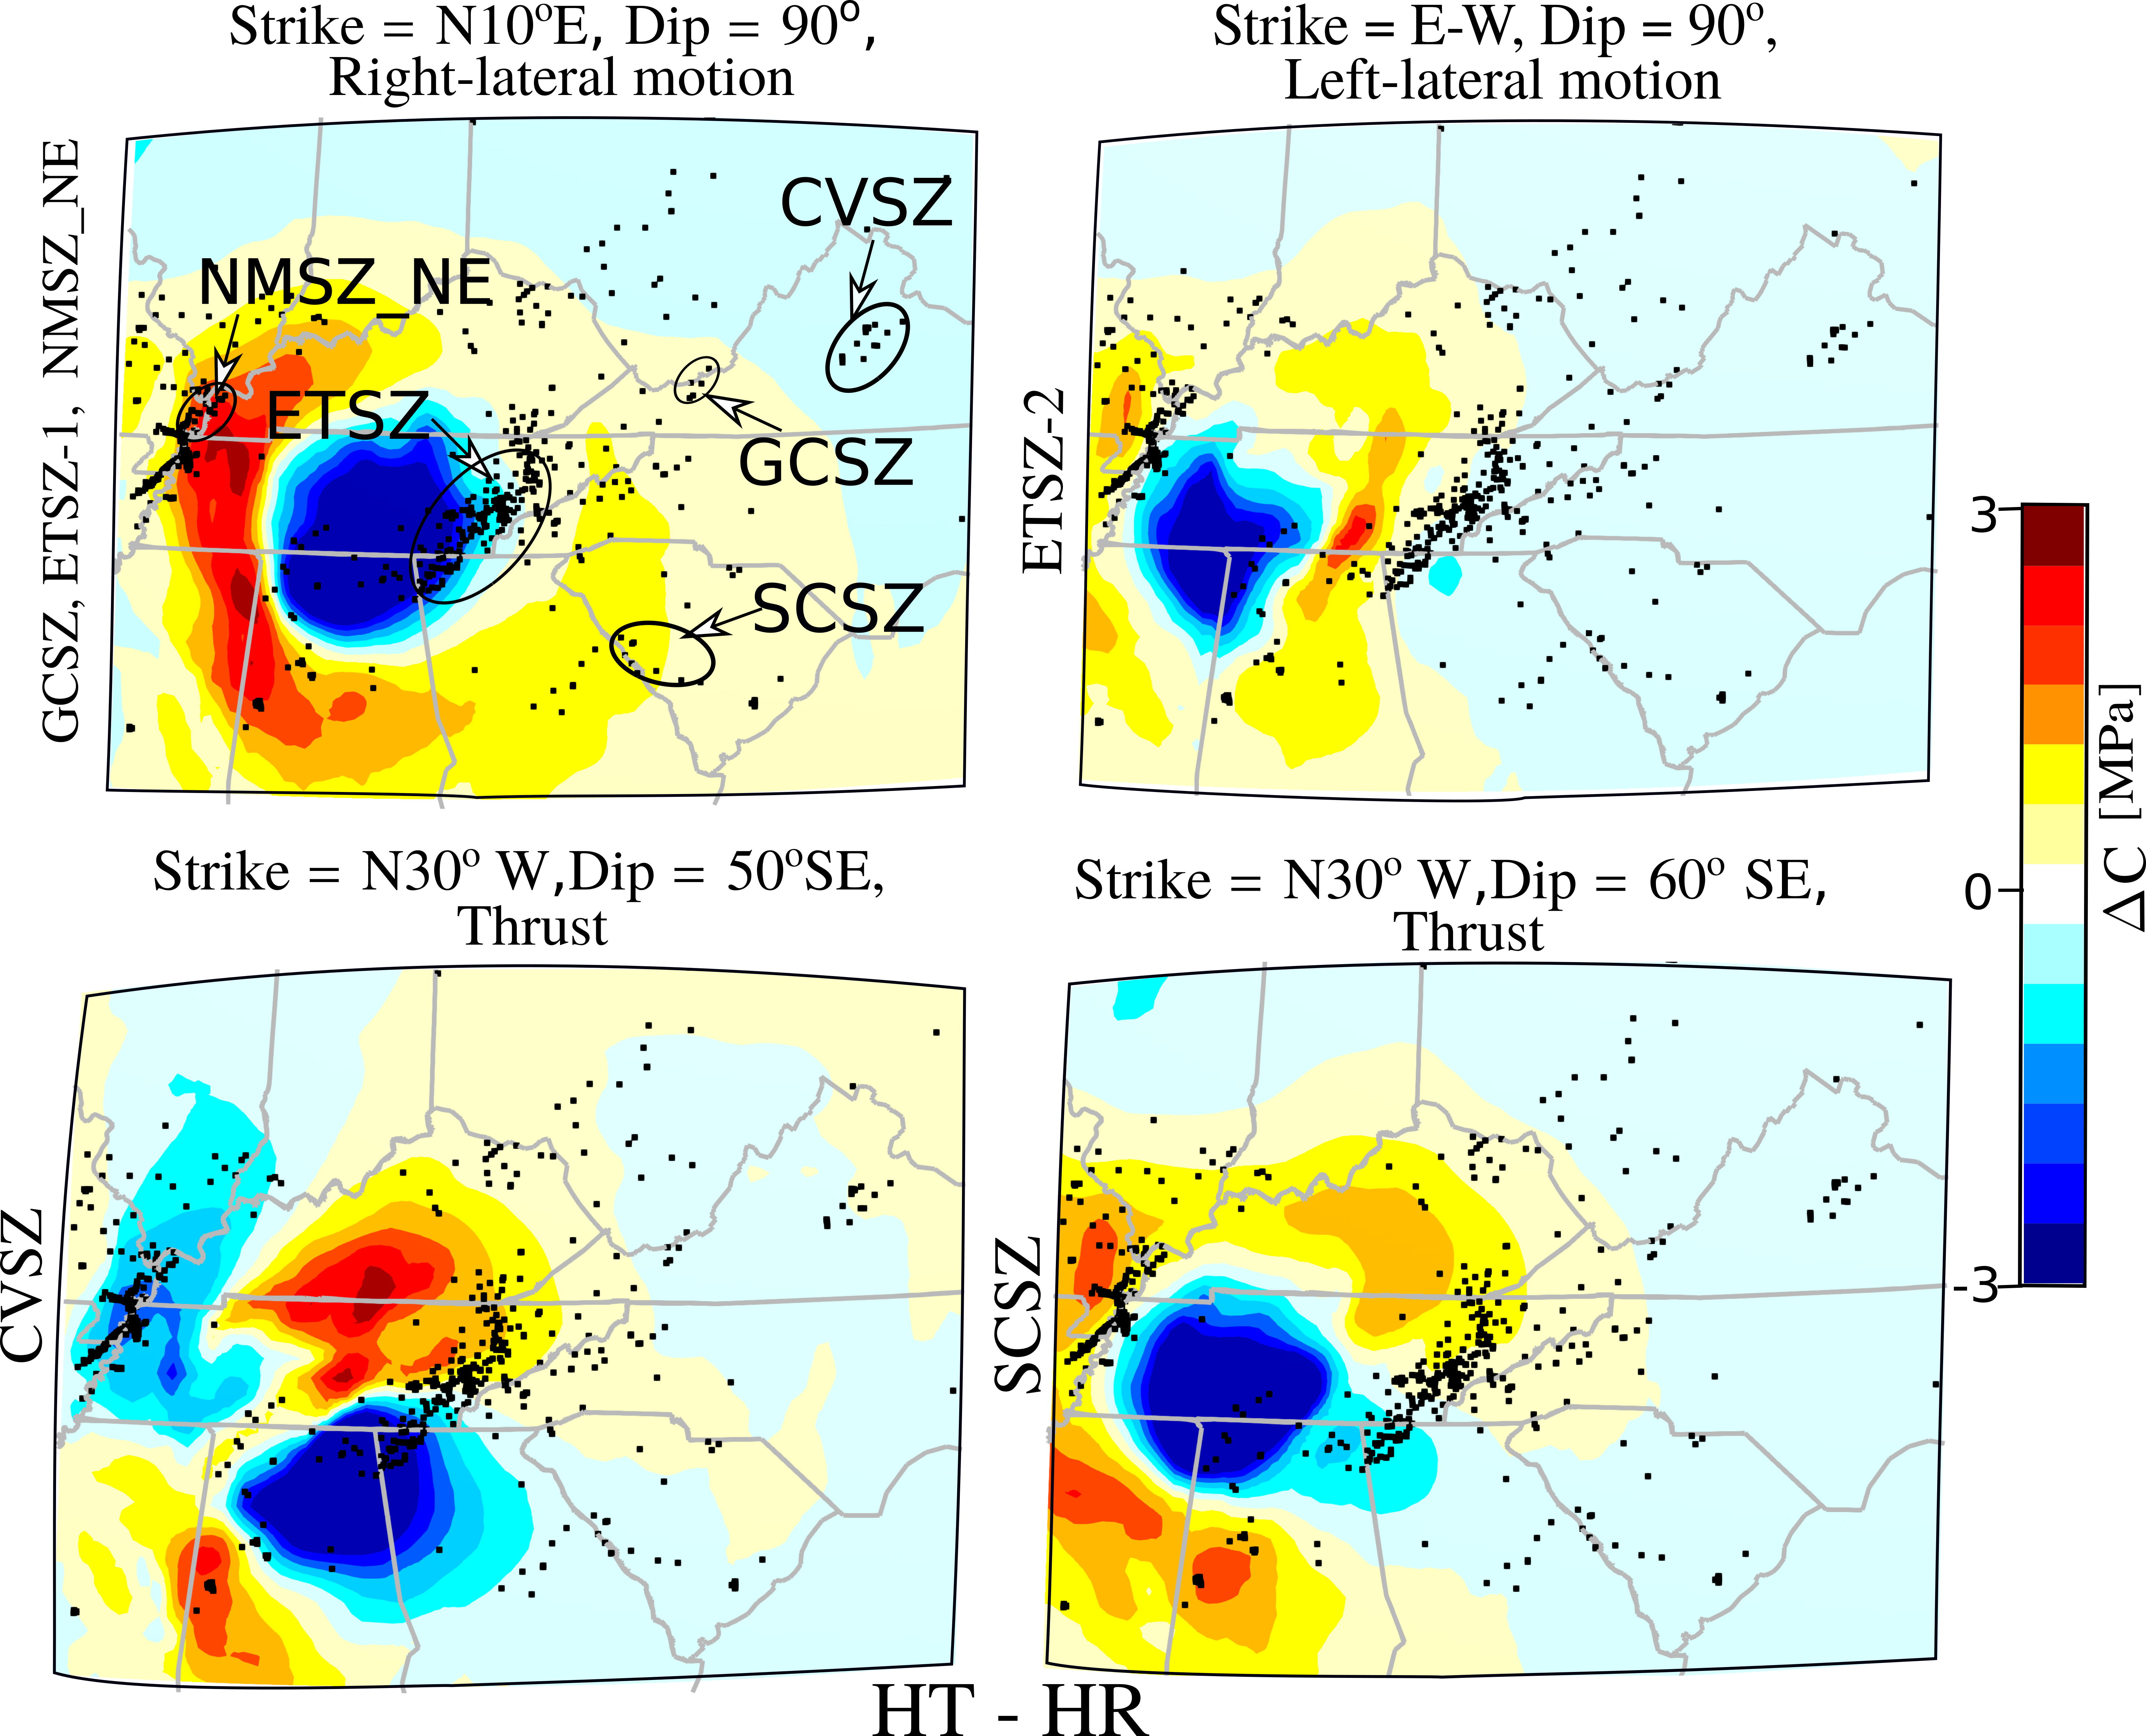
\includegraphics[width=0.75\linewidth]{figures/cs_ht_hr.png}
    \caption{Same as Fig.~\ref{ht_hm_cs} but for HT$-$HR.}
    \label{ht_hr_cs}
\end{figure}

%The results from Fig.~\ref{ht_hm_cs} and Fig.~\ref{ht_hr_cs} are reflected in the calculated slip coefficient values, $\Theta$, which measures the fraction of model node points within each seismic zone that could slip. Fig.\ref{ht_hm_corr} shows the $\Theta$ for each seismic zone at their optimal fault geometry. A perfect correlation of increased $\Delta C$ with the points within the GCSZ is observed ($\Theta$ = 1) when all the upper mantle heterogeneity is considered (HT$-$HM), while no points within the GCSZ show a tendency to slip when only effects of the drip are considered (HT$-$HR). For the two optimal fault planes considered for the ETSZ (see Table  \ref{table_fault}), fault-2, (i.e., left-lateral vertical fault striking EW), promotes a higher number of points within the ETSZ to slip for both model setups: HT$-$HR, HT$-$HM. On the contrary, all the points within the NMSZ and the CVSZ lie in the $\Delta C$ shadow giving zero slip coefficient for HT$-$HM and HT$-$HR. Some points within the SCSZ show a small tendency to slip for the model HT$-$HR but no tendency for the HT$-$HM model (Fig.~\ref{ht_hm_corr}).
%%
%\begin{figure}[h!]
%    \centering
%    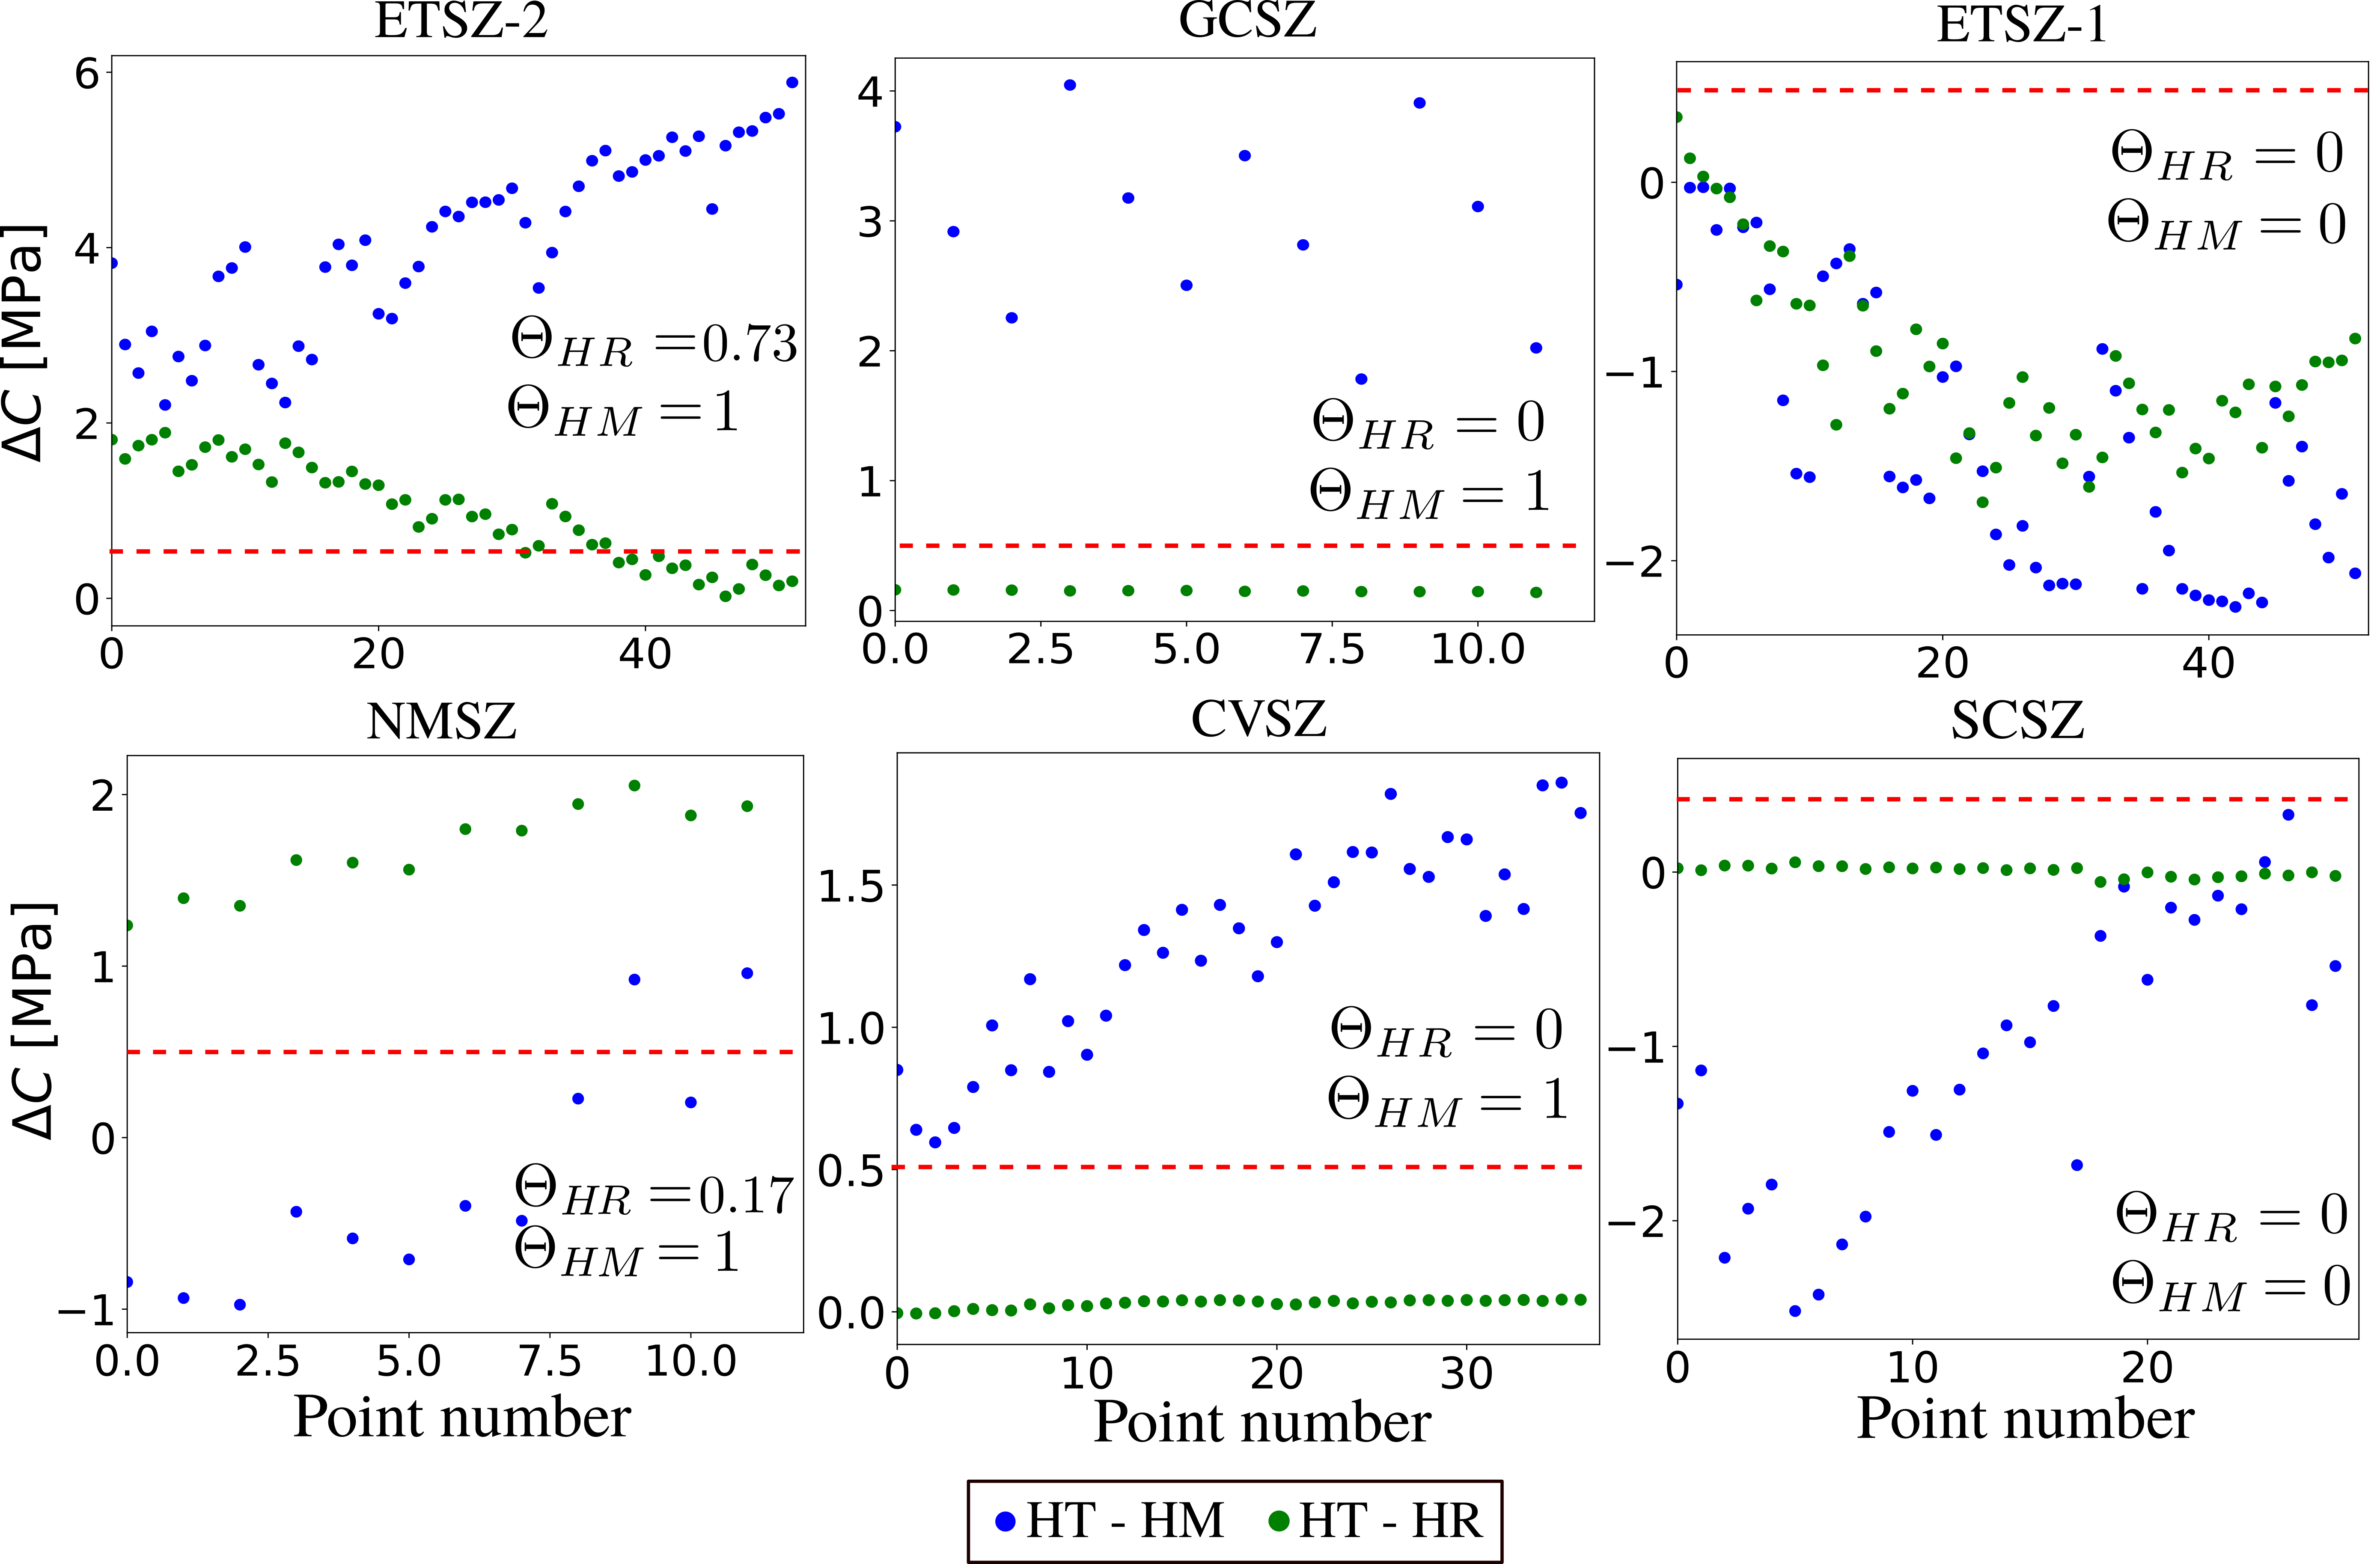
\includegraphics[width=0.75\linewidth]{figures/corr_cs.png}
%    \caption{Coulomb stress changes ($\Delta C$) in the case HT$-$HM and HT$-$HR  at selected points in the model corresponding to the epicenters of the seismic zones at the NMSZ, ETSZ, CVSZ, SCSZ and GCSZ. $\Delta C$ is computed for the respective optimal fault orientations listed in Table~\ref{table_fault} and at 15 km depth. The dashed red line denotes the $\Delta C$ = 0.5 MPa threshold. Each panel is annotated with $\Theta$ value, the fraction of points above 0.5 MPa in a seismic zone.}
%    \label{ht_hm_corr}
%\end{figure}


%
    %%%%%
\section{Discussion and Summary}
%    In this study, we investigate the stress effects due to upper mantle heterogeneity, $>$ 200 km depth, and isolated lithospheric instability on the intraplate seismicity of the CEUS using numerical models based on the temperatures calculated from the \citet{Biryol_2016} tomography results. Many possible stress concentrators in the CEUS have been proposed to explain the seismicity \citep[e.g.,][]{levandowski2016dense, zhan2016stress} but analysis done here invoking deeper upper mantle structures and impact collectively on the seismicity in the CEUS has not been done before. 
    
    
Changes in differential stress ($\Delta \sigma_{\text{diff}}$) and the Coulomb stress ($\Delta$C) for the cases HT$-$HM and HT$-$HR quantify how the upper-mantle heterogeneity and the lithospheric drip, respectively, can contribute to the seismicity in the ETSZ, GCSZ, CVSZ, SCSZ and NMSZ (see Fig. \ref{figone} for their locations).
$\Delta\sigma_{diff}^{\text{HT}-\text{HM}}$ involves the combined effects of all the mantle heterogeneities relative to the laterally homogeneous reference mantle and shows positively values up to 30 MPa in all of the seismic zones considered (Fig.~\ref{df_model}a). On the other hand, The lithospheric drip alone has an area of influence that includes only the ETSZ and NMSZ as $\Delta\sigma_{diff}^{\text{HT}-\text{HR}}$ %and $\Delta$C$_{\text{HT}-\text{HR}}$ 
shows positive values of about 3 MPa only in the ETSZ and NMSZ\_NE. Although the positive values of differential stress changes suggest an increased potential for seismicity, even the greatest value of $\Delta\sigma_{diff}^{\text{HT}-\text{HM}}$, $\sim$ 30 MPa in the ETSZ, is an order of magnitude less for that required for the nucleation of earthquakes at crustal depths of 10-20 km~\citep[e.g.][]{sibson1990rupture}. This deficiency in magnitude require other contributions for explaining the seismicity in the CEUS like weak existing faults created during the past continental rifting events during the several Wilson cycles~\citep{thomas2006tectonic}). From our Coulomb stress change calculations for the optimal fault geometries of the seismic zones (Table~\ref{table_fault}), we find that these faults are more loaded towards failure  in the hetetogeneous upper mantle revealed by the tomography than in the laterally uniform one.
       
%     The location of the foundering drip has a significant impact on concentrating the differential stress at the surrounding seismic zones, the ETSZ and the NMSZ. We considered a model with the drip shifted to the east such that it begins below the ETSZ and not between the NMSZ and the ETSZ. The stress increase for the shifted root model surrounds the ETSZ and does not correlate with any observed seismic zones. We also setup synthetic models including viscosity layers for the crust, lithosphere, and asthenosphere with a region of laterally thickened lithosphere and calculated stress changes with respect to a model with laterally uniform lithospheric thickness. Our computations suggested that stress concentration occurs at the boundary of large lateral viscosity change (2 to 3 orders magnitude). Since the viscosities are computed based on the temperatures inverted from the Vp anomalies, our results indicate that the stress concentration occurs along the edges of high-velocity anomalies, which has been previously proposed by~\citet{zhang2009tomographic}. 
    
    %The Coulomb stress change is calculated at the selected fault orientations determined from previous studies on focal mechanism and earthquake hypocentral relocation in these seismic zones \citep[e.g.,][]{cooley2015new, powell2016grenville, munsey1985focal, chiu1992imaging}. In HT$-$HM, ETSZ, GCSZ and northeastern arm of NMSZ show an increase in Coulomb stress for the proposed fault orientation in these regions and CVSZ shows a weak positive increase while SCSZ overlies in the stress shadow, i.e. negative Coulomb stress change. Conversely, HT$-$HR does not show strong correlation between seismiciy and the Coulomb stress increase at all seismic zones except NMSZ.
    
     We find the optimal fault orientations for the stress fields determined by our models. Defining the optimal orientation as the one maximizing the Coulomb stress changes of HT relative to HM or HR, we employ a simple grid search over strikes from N$90^\circ$E to S$90^\circ$E and dips from 10$^\circ$ to 90$^\circ$     % at intervals of $10^\circ$, for 
     for each of the possible senses of motion, right-lateral and left-lateral strike-slip, normal and thrust faulting. 
%     We only show fault orientations between E-W and NNW-SSE because the orientations of the faults in the seismic zones are confined within this range according to previous studies~\citep{shumway2008focal, hurd2012intraplate, johnson2014earthquake, cooley2015new}. 
     Results for HT$-$HM are shown in Fig. S1 and those for HT$-$HR in Fig.~S1. Since the effects of the drip are spatially limited to the ETSZ and the NMSZ (Fig.~S2) and are smaller in magnitude compared to HT$-$HM (Fig. S2), we identify the most optimally orientated fault plane as the orientation and sense of motion where $\Delta$C$_{HT-HM}$ is maximized.
 %    
%\begin{figure}[ht]
%    \centering
%    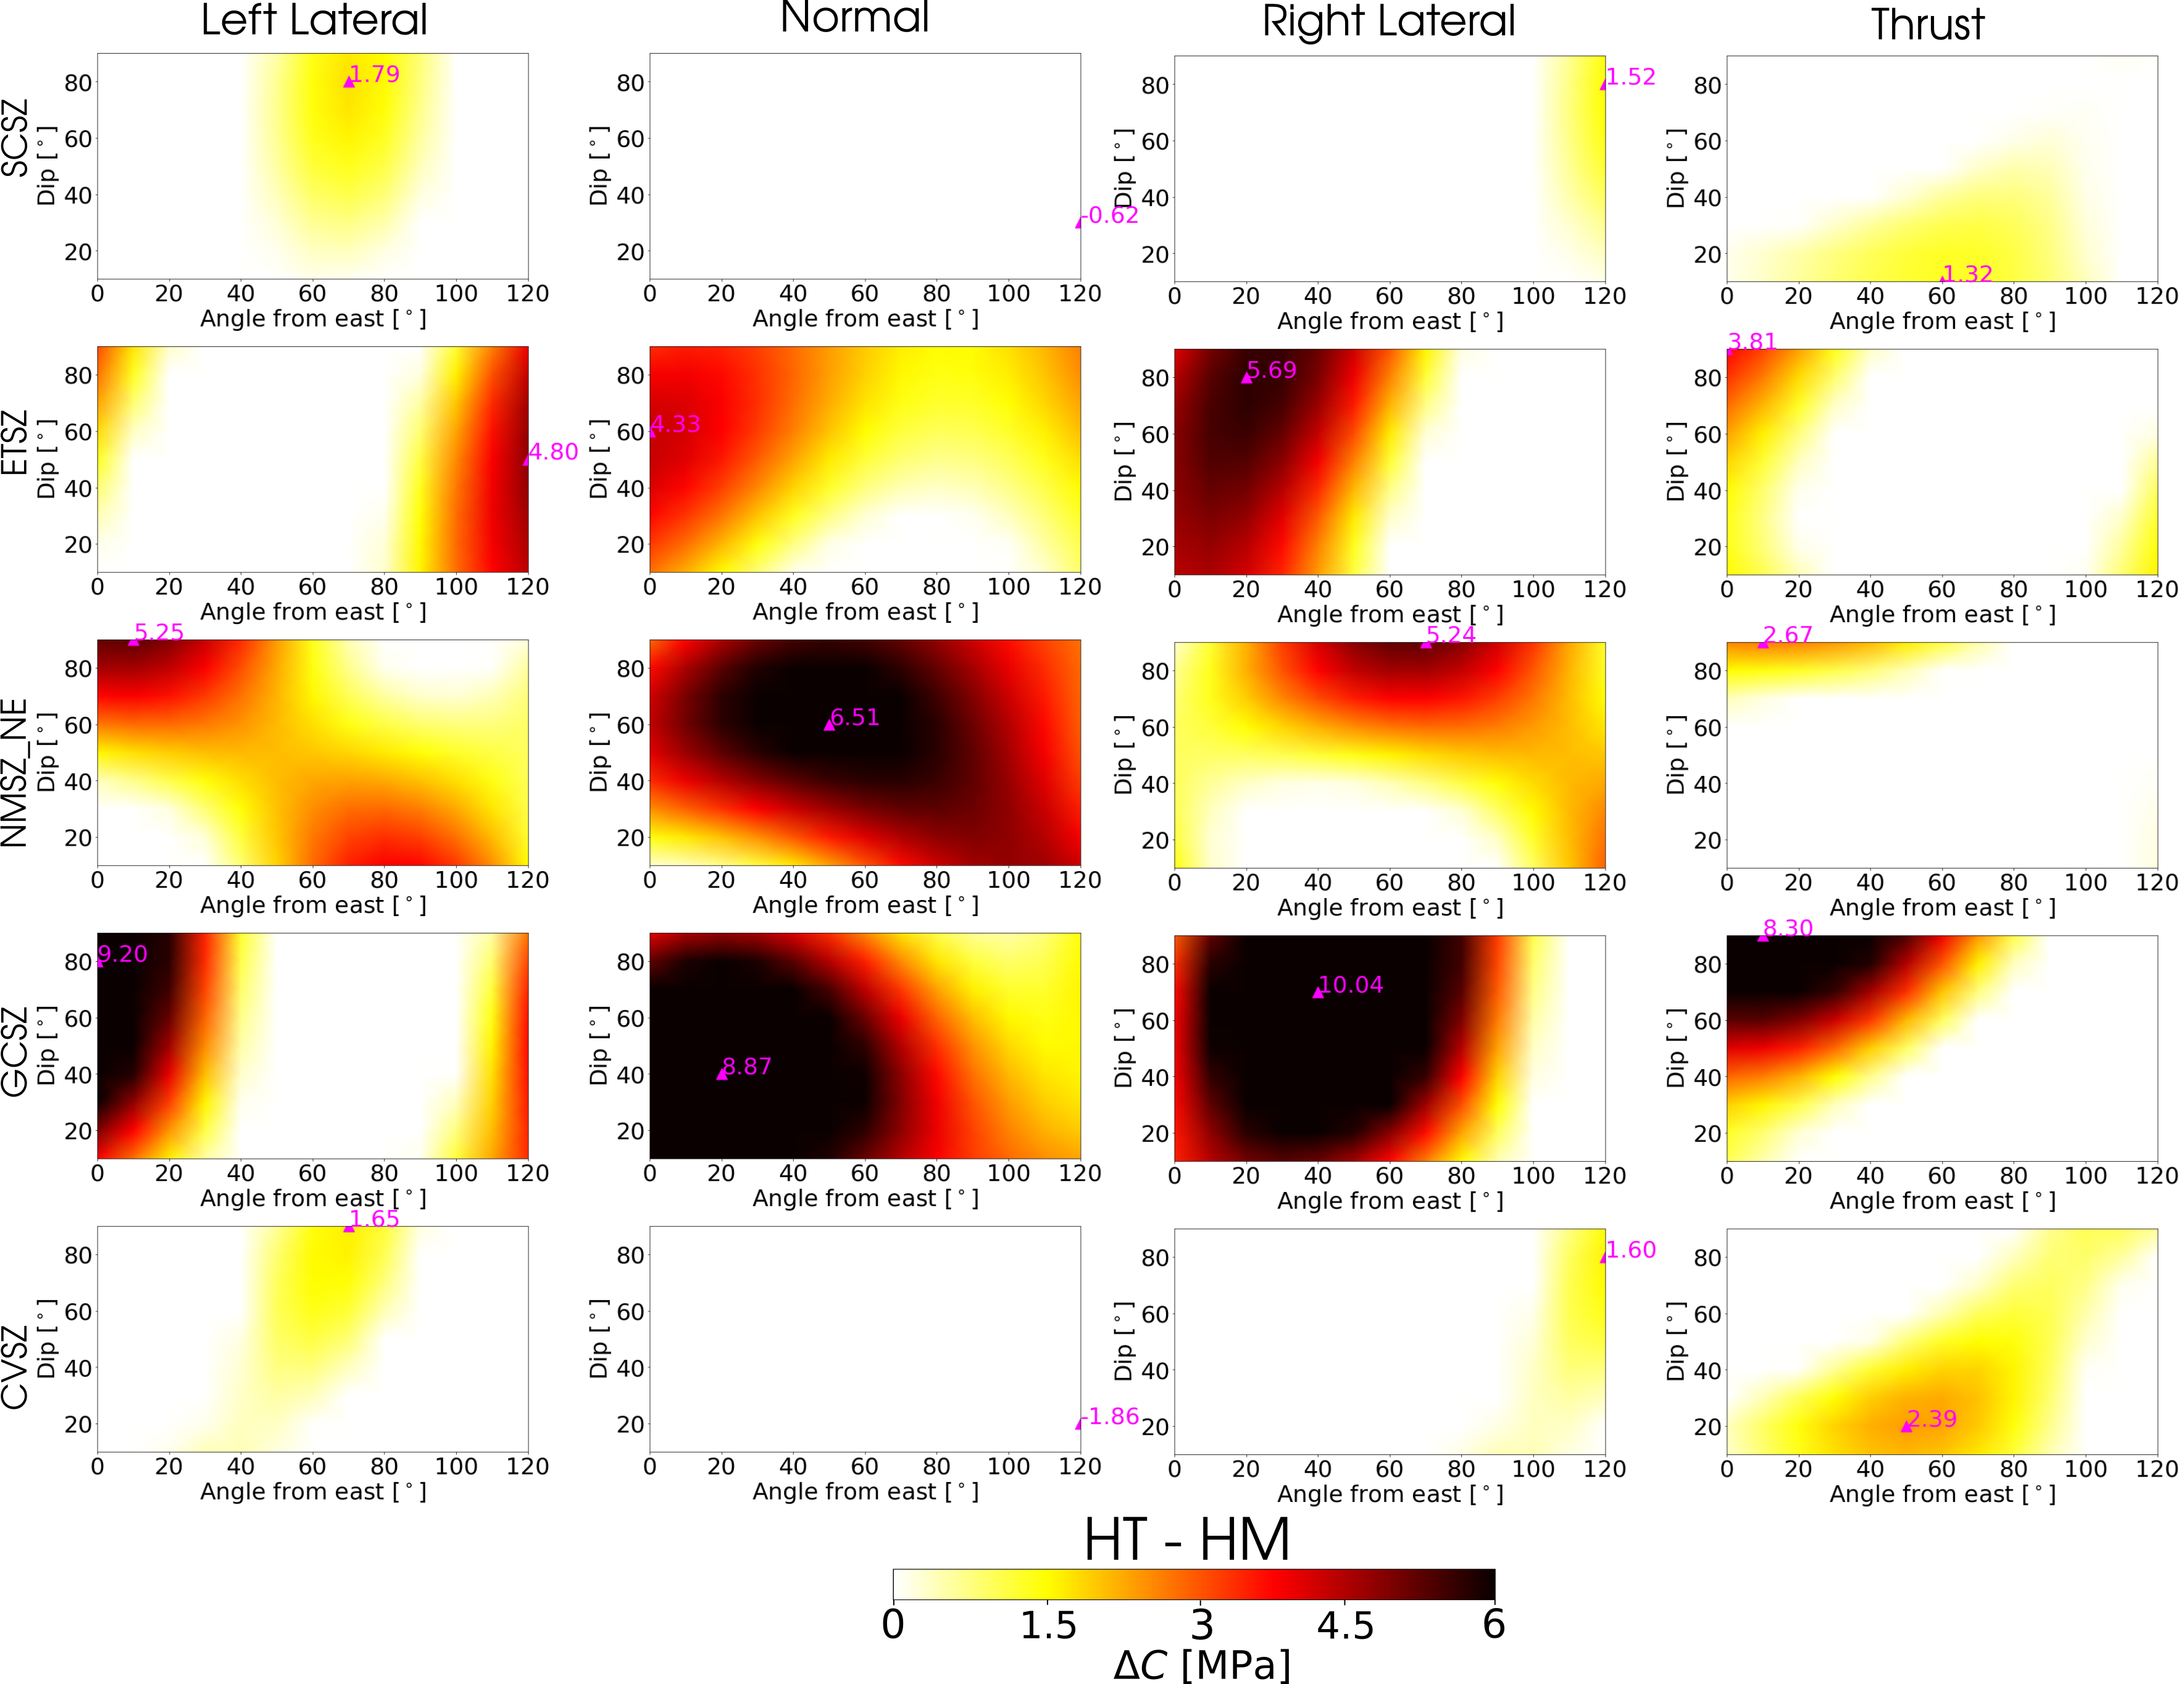
\includegraphics[width=\linewidth]{figures/ht_hm_summ.png}
%    \caption{Coulomb stress change for HT$-$HM in the seismic zones for possible strikes, dips, and slip directions: right-lateral, left-lateral strike-slip, normal, and thrust faulting. Subplots are also labeled with maximum $\Delta C$, and a triangular marker denoting the orientation and dip where the maximum occurs.}
%    \label{cs_ht_hm}
%\end{figure}
%%
%\begin{figure}[ht]
%    \centering
%    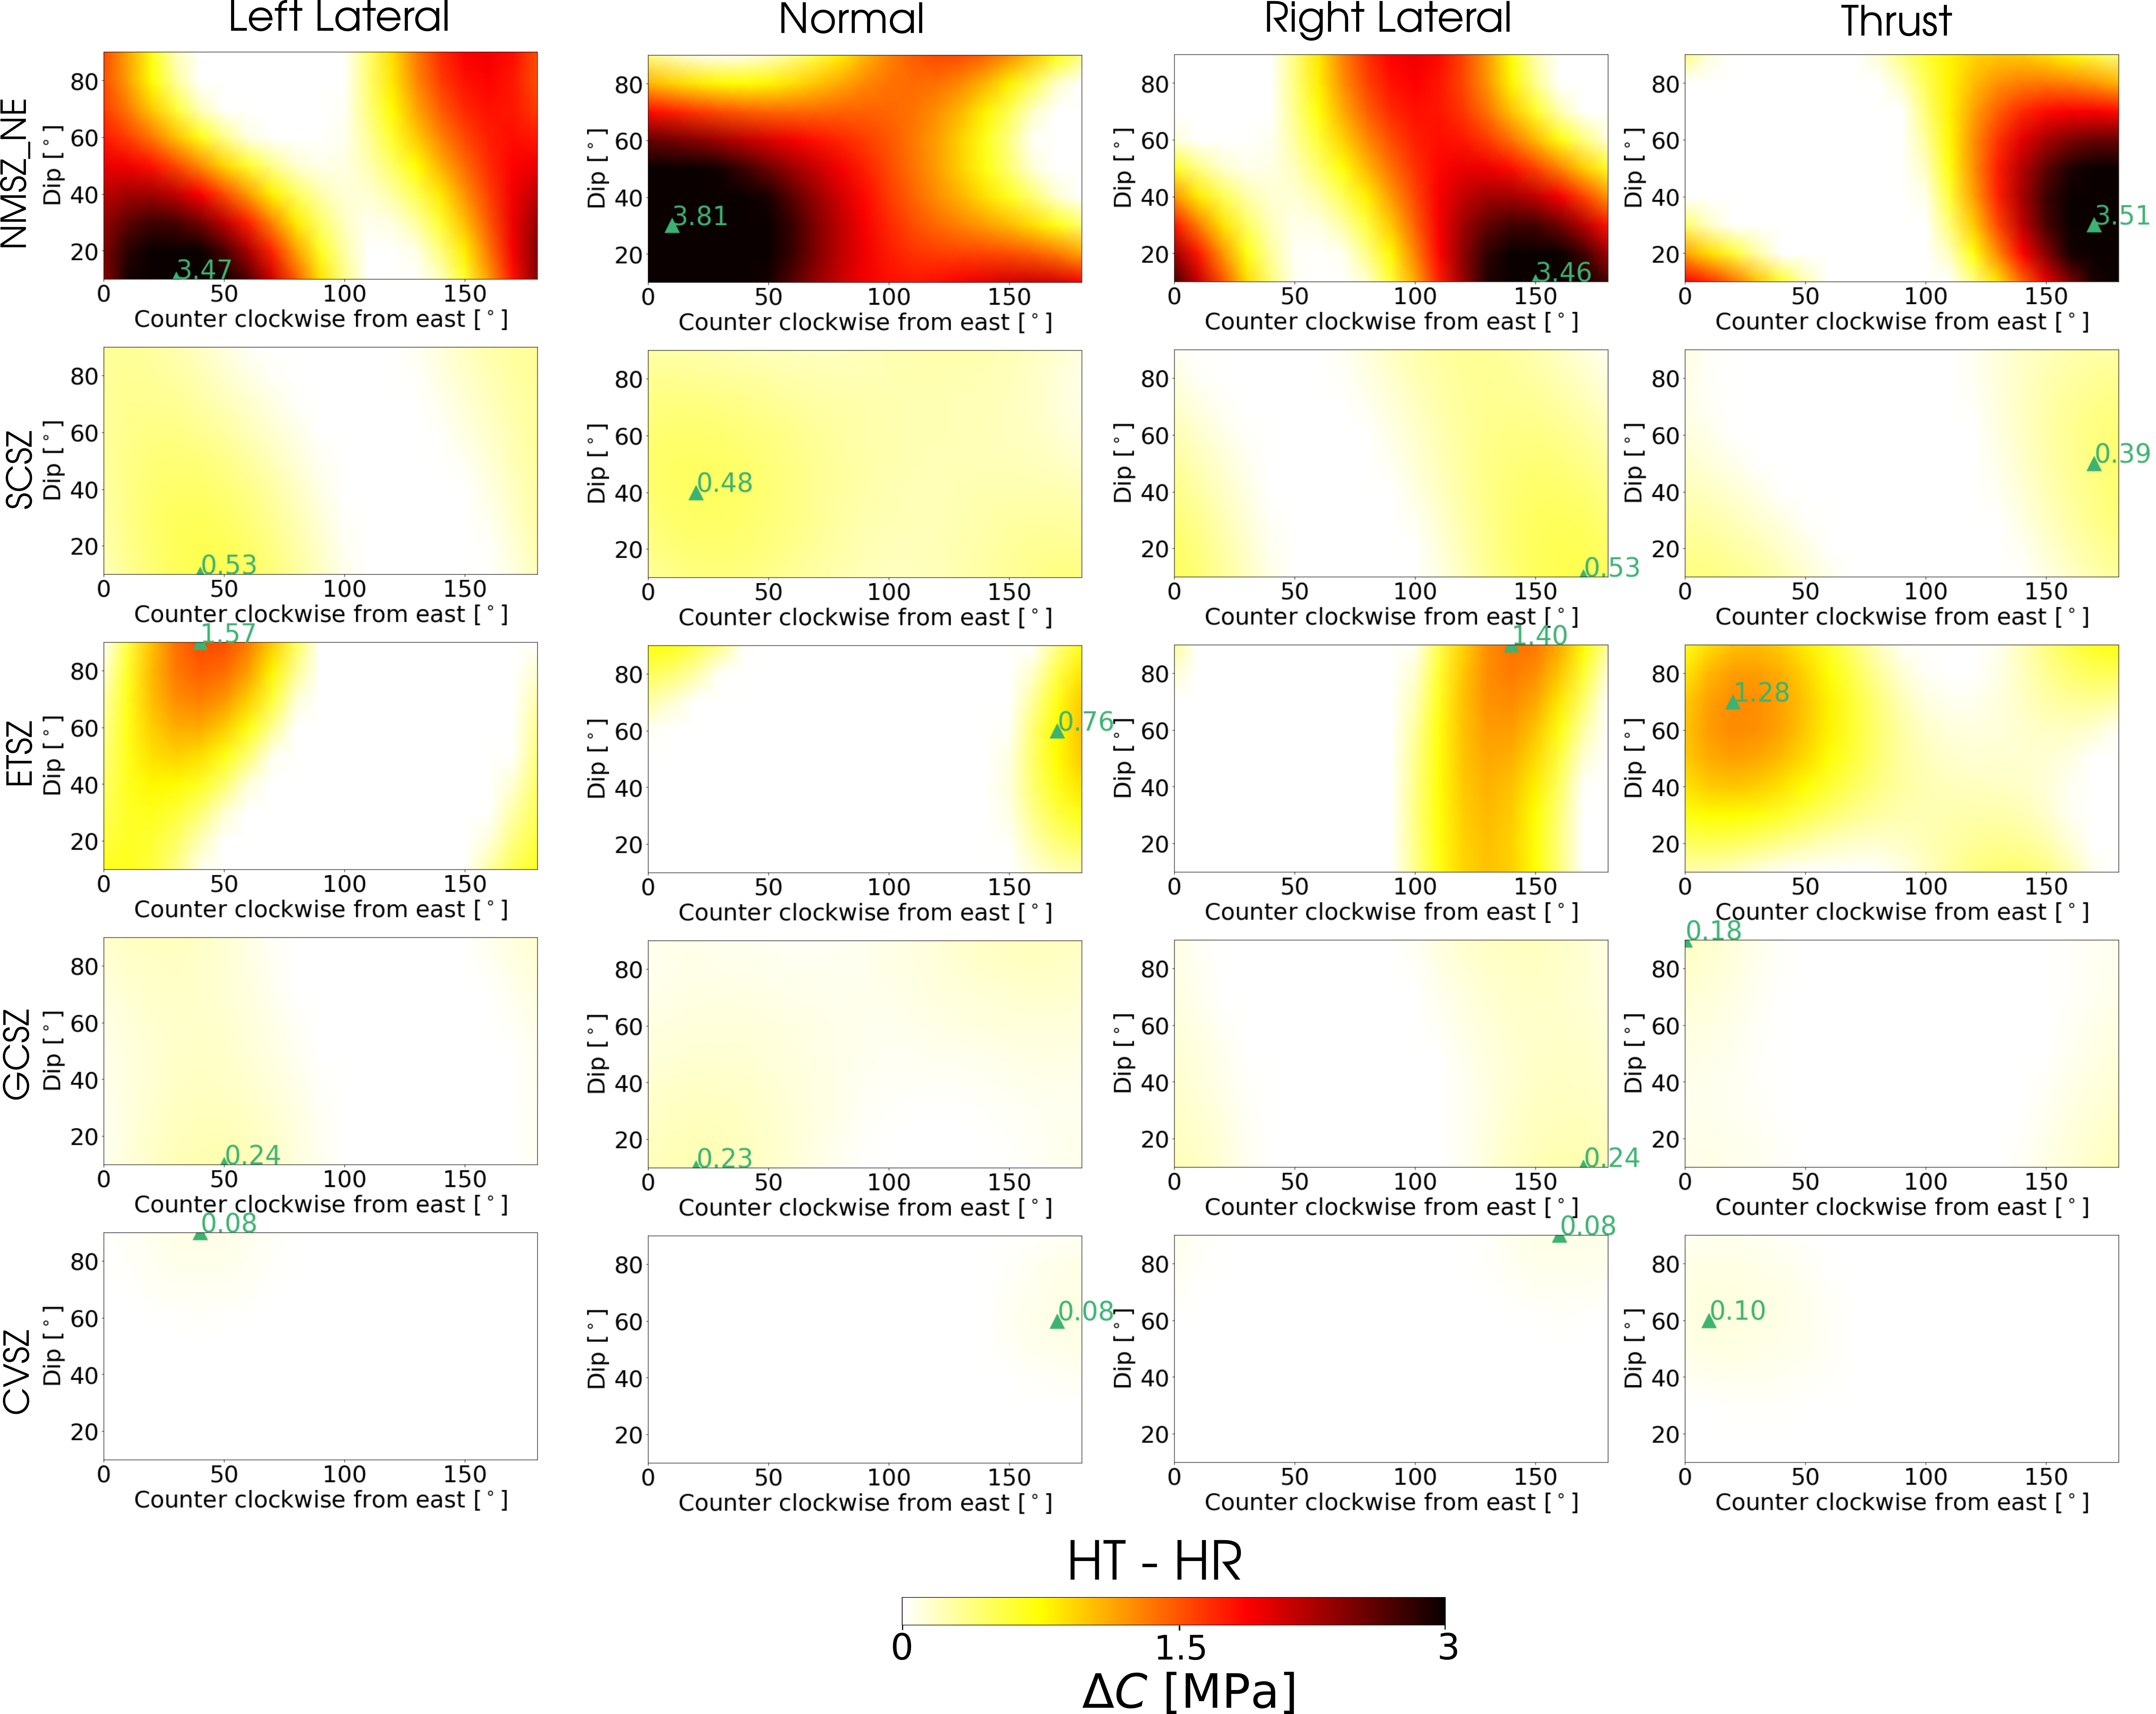
\includegraphics[width=\linewidth]{figures/ht_hr_summ.png}
%    \caption{Same as in Fig. \ref{cs_ht_hm} but for HT$-$HR.}
%    \label{cs_ht_hr}
%\end{figure}

     The most optimally oriented fault planes in Fig.~S1 based on our model results do not coincide with the proposed focal mechanism solutions in the seismic zones (Fig.~\ref{summary}). There are several reasons for the mismatch. Firstly, the focal mechanisms investigated in this study for each of the seismic zones are not unique; there are other proposed focal mechanisms documented in the literature, but we only select focal planes for each seismic zone that are most prevalent. Moreover, at some seismic zones such as the SCSZ and the CVSZ, the seismicity is diffuse so that a single mechanism cannot describe the entire zone~\citep{johnson2014earthquake, munsey1985focal, madabhushi1993fault}.  Secondly, the presence of upper mantle heterogeneity is not the only contributing factor for stress concentration in the CEUS. Other factors such as a dense sinking body in a weak lower crust as proposed by \citet{Pollitz_2001} or weak lower crust or upper mantle embedded in an elastic lithosphere by \citet{Kenner_2000a} or isostatic response from deglaciation of Laurentia by ~\citet{Grollimund_2001}, may also play a role at shallower depths.  Thirdly, most of the earthquakes in the CEUS occur at depths $<$ 20 km~\citep[e.g.,][]{bollinger1985seismicity, chiu1992imaging, powell2016grenville} on reactivated faults formed from one or two Wilson cycles~\citep{thomas2006tectonic, wolin2012mineral}. The mantle tomography model in our study does not provide constraints on the geometry and strength of the shallow seismogenic faults created in the past. Lastly, our model does not account for any tectonic stresses since our focus is on the local stress perturbations from the upper mantle. In reality, the effects of plate motion, as included by~\citet{zhan2016stress} and \citet{levandowski2016dense}, will influence the near-surface stress field.% When taken into account, together or alone, all of these factors might bring the optimal orientations closer to those independently estimated in the previous studies.
Therefore it can be inferred that the presence of mantle heterogeneity is a factor in generation of the earthquakes but not the sole factor and the mantle heterogeneity should be accounted for in any comprehensive model of earthquake generation.
     
\begin{figure}[ht]
    \centering
    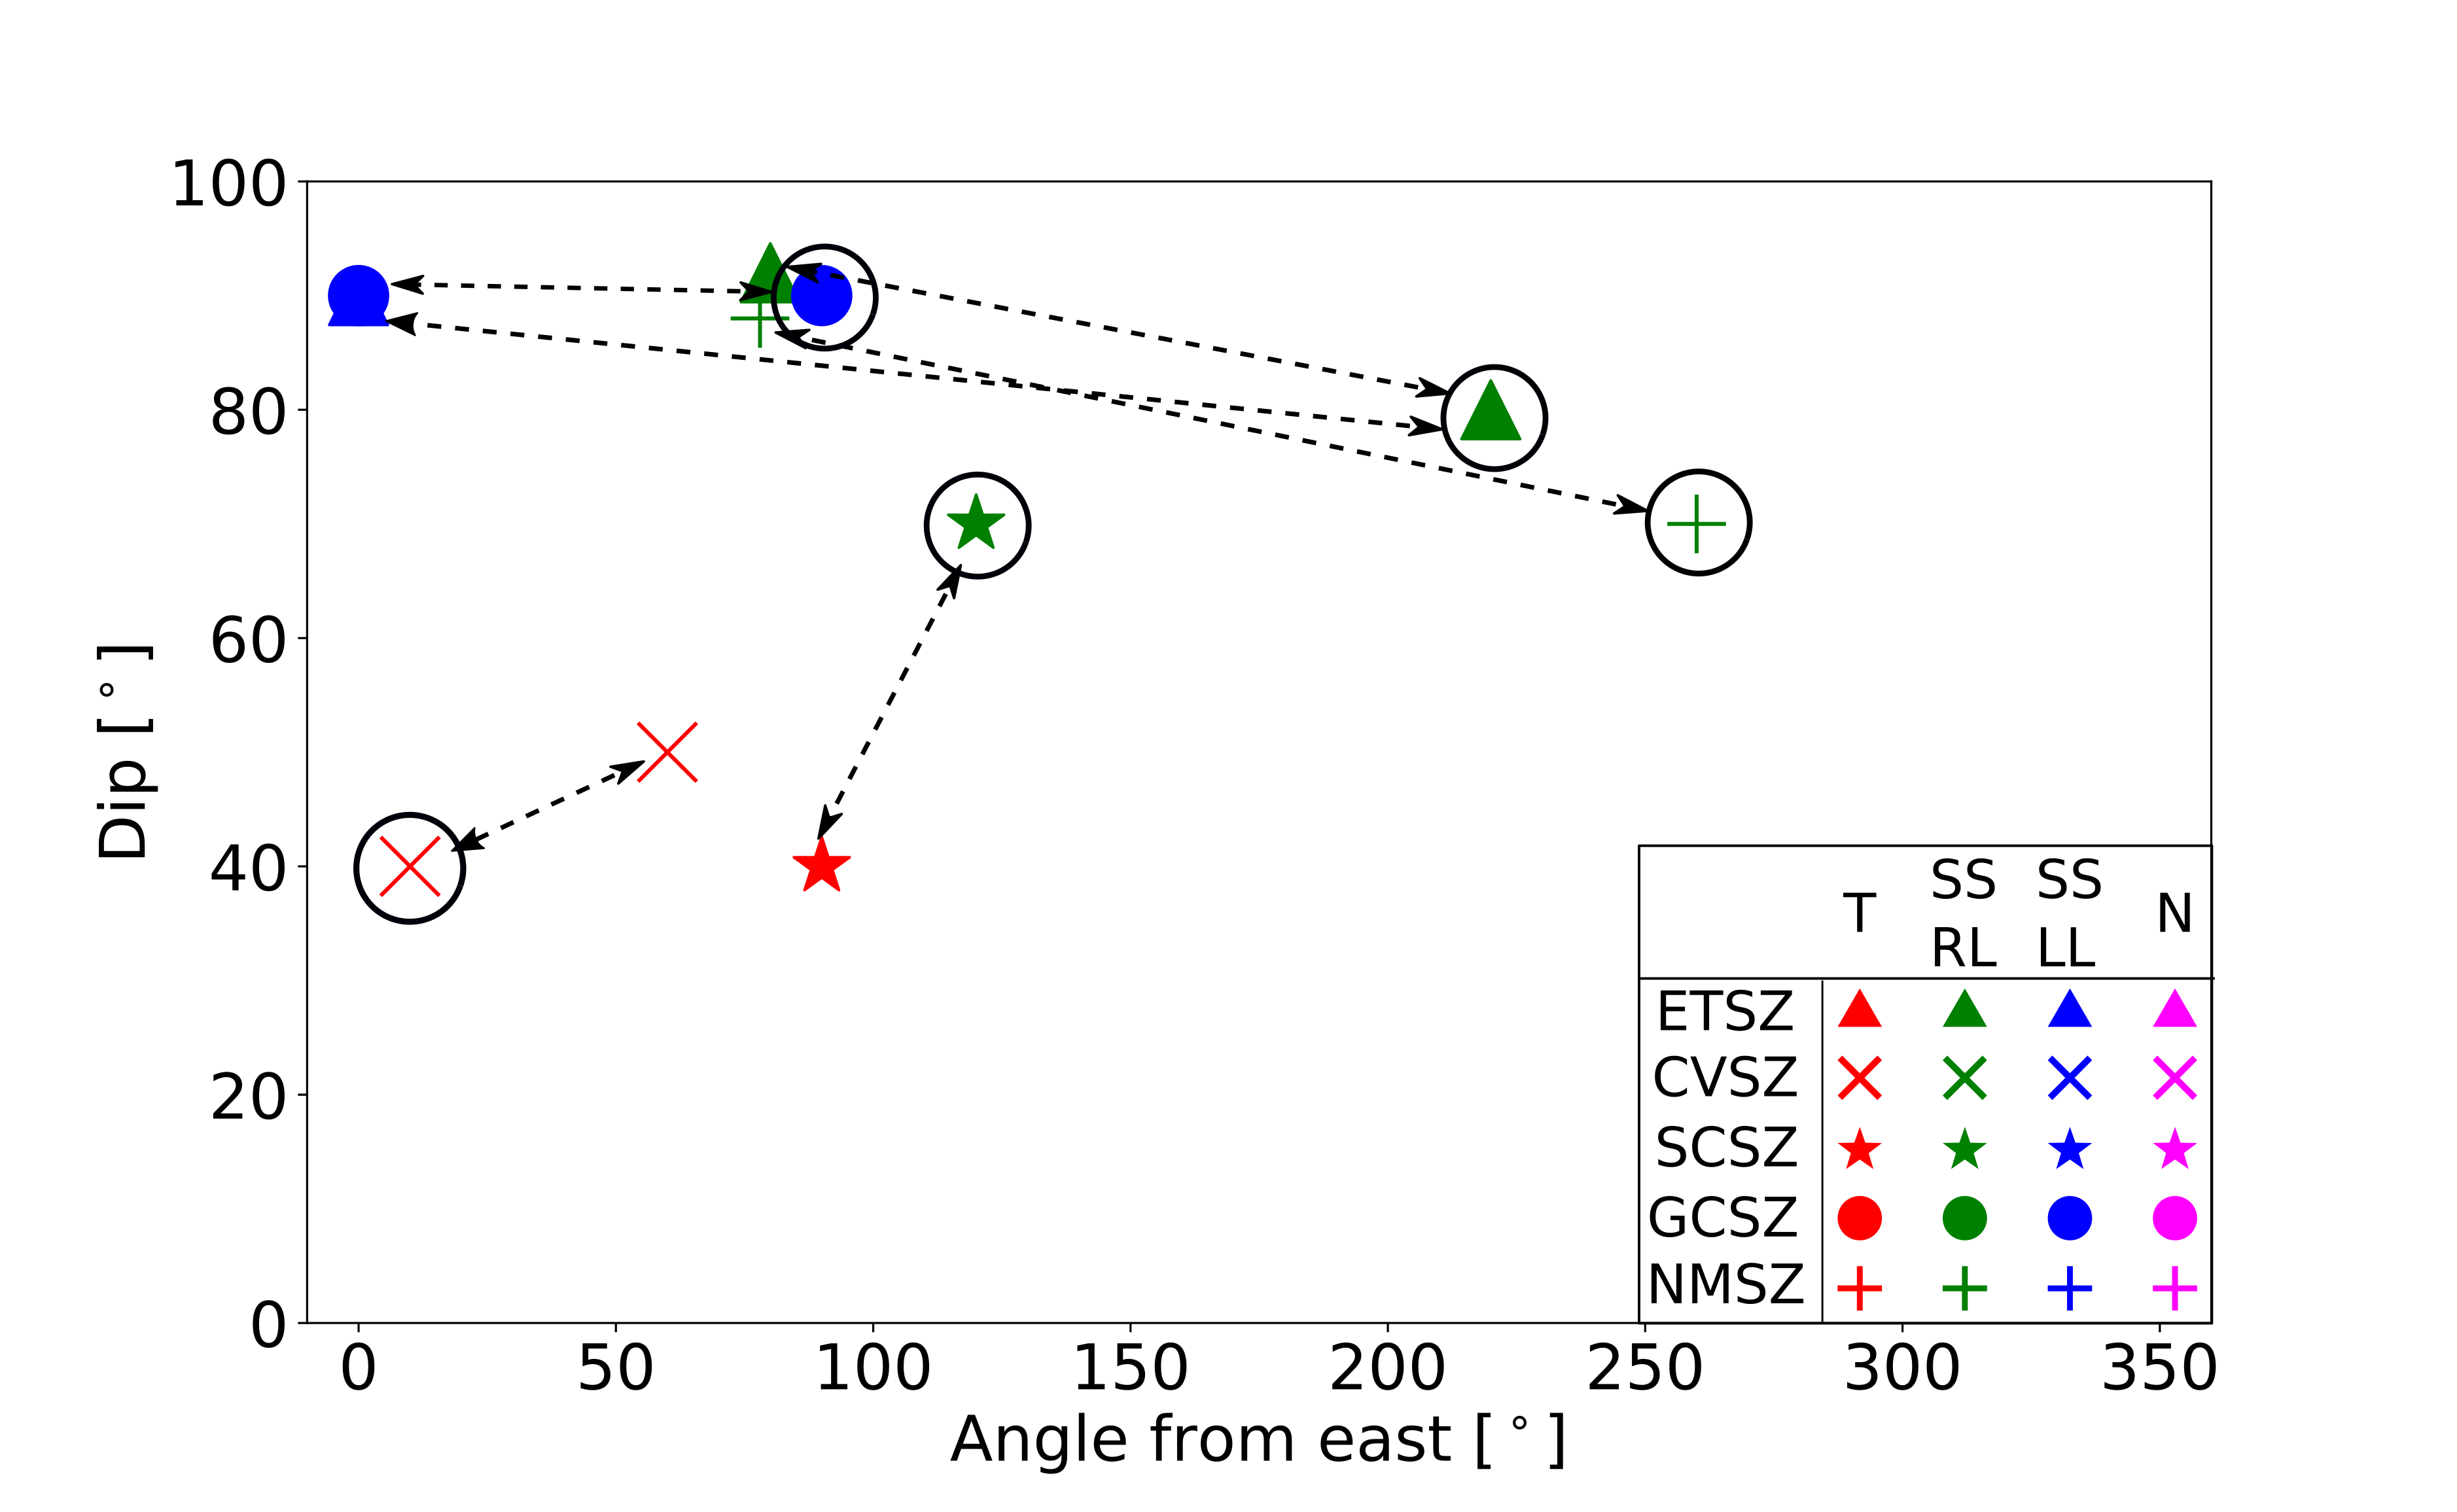
\includegraphics[width=0.8\linewidth]{figures/summ_stress.png}
    \caption{Proposed fault planes from other studies based on focal mechanism and earthquake hypocenters versus fault planes at which $\Delta$C$_{HT-HM}$ is maximum. The markers represent each of the seimic zones: New Madrid Seismic Zone (NMSZ), Eastern Tennessse Seismic Zone (ETSZ) South Carolina Seismic Zone (SCSZ), Giles County Seismic Zone (GCSZ) and Central Virginia Seismic Zone (CVSZ). The sense of fault slip is indicated with the color of the marker as thrust(T), right-lateral strike-slip (SS, RL), left-lateral strike slip (SS, LL) and normal (N). 'M' denoted near the marker represents the orientation at which $\Delta$C$_{HT-HM}$ is maximum in the model.}
    \label{summary}
\end{figure}
 
     %The important result of our study is the increase in the Coulomb stress in the active CEUS seismic zones due to the presence of the upper mantle heterogeneity.
%    which is computed using $R'=(\sigma_2-\sigma_3)/(\sigma_1-\sigma_3)$ (here, $\sigma_1>\sigma_2>\sigma_3$ are the principal stress components and $\sigma_1$ is most compressive), and the faulting style


We compute the maximum horizontal stress directions (S$_H$) and faulting style for our tomography-based heterogeneous model, HT, in Fig.~\ref{sigma1} and compare them with the proposed S$_H$ and faulting style from a recent stress inversion study by~\citet{levandowski2018updated}. We calculate the  stress regime parameter, $R$,~\citep{delvaux1997paleostress}, as done by~\citet{levandowski2018updated}. R varies from 0 for radial extension, through normal, strike-slip, and reverse faulting to radial contraction at R=3~\citep{delvaux1997paleostress, simpson1997quantifying}. The S$_H$ computed from our model roughly matches with the S$_H$ obtained by~\citet{levandowski2018updated} for all the seismic zones except the ETSZ.  Our computed NNW-SSE SH for the ETSZ differs from the NE-SW SH direction determined using focal mechanism solutions by~\citet{levandowski2018updated} and by~\citep{mazzotti2010state}. This is not surprising as faulting in the ETSZ may be strongly influenced by density anomalies in the lower crust inherited from past tectonic events~\citet{levandowski2018updated}. This is suggested by the occurrence of focal mechanisms indicating a propensity for normal faulting in the ETSZ~\citep{cooley2015new}. Fig.~\ref{sigma1} shows the dominant faulting style as thrust for the NMSZ, and oblique-thrust for the GCSZ, which is similar to the proposed faulting styles in~\citet{levandowski2018updated} for these zones. On the other hand, our model predicts normal faulting at the SCSZ and the CVSZ, and strike-slip faulting at the ETSZ. These zones are associated with thrust and normal faulting, receptively, in~\citet{levandowski2018updated}. This discrepancy between the modeled and predicted faulting style at the CVSZ and the SCSZ occurs because our model does not account for compressive tectonic stresses, which is highest at these zones. Within the ETSZ, a strike-slip mechanism has been dominantly suggested by other studies~\citep{mazzotti2010state, powell2016grenville}, which agrees with our model result.

\begin{figure}[h!]
    \centering
    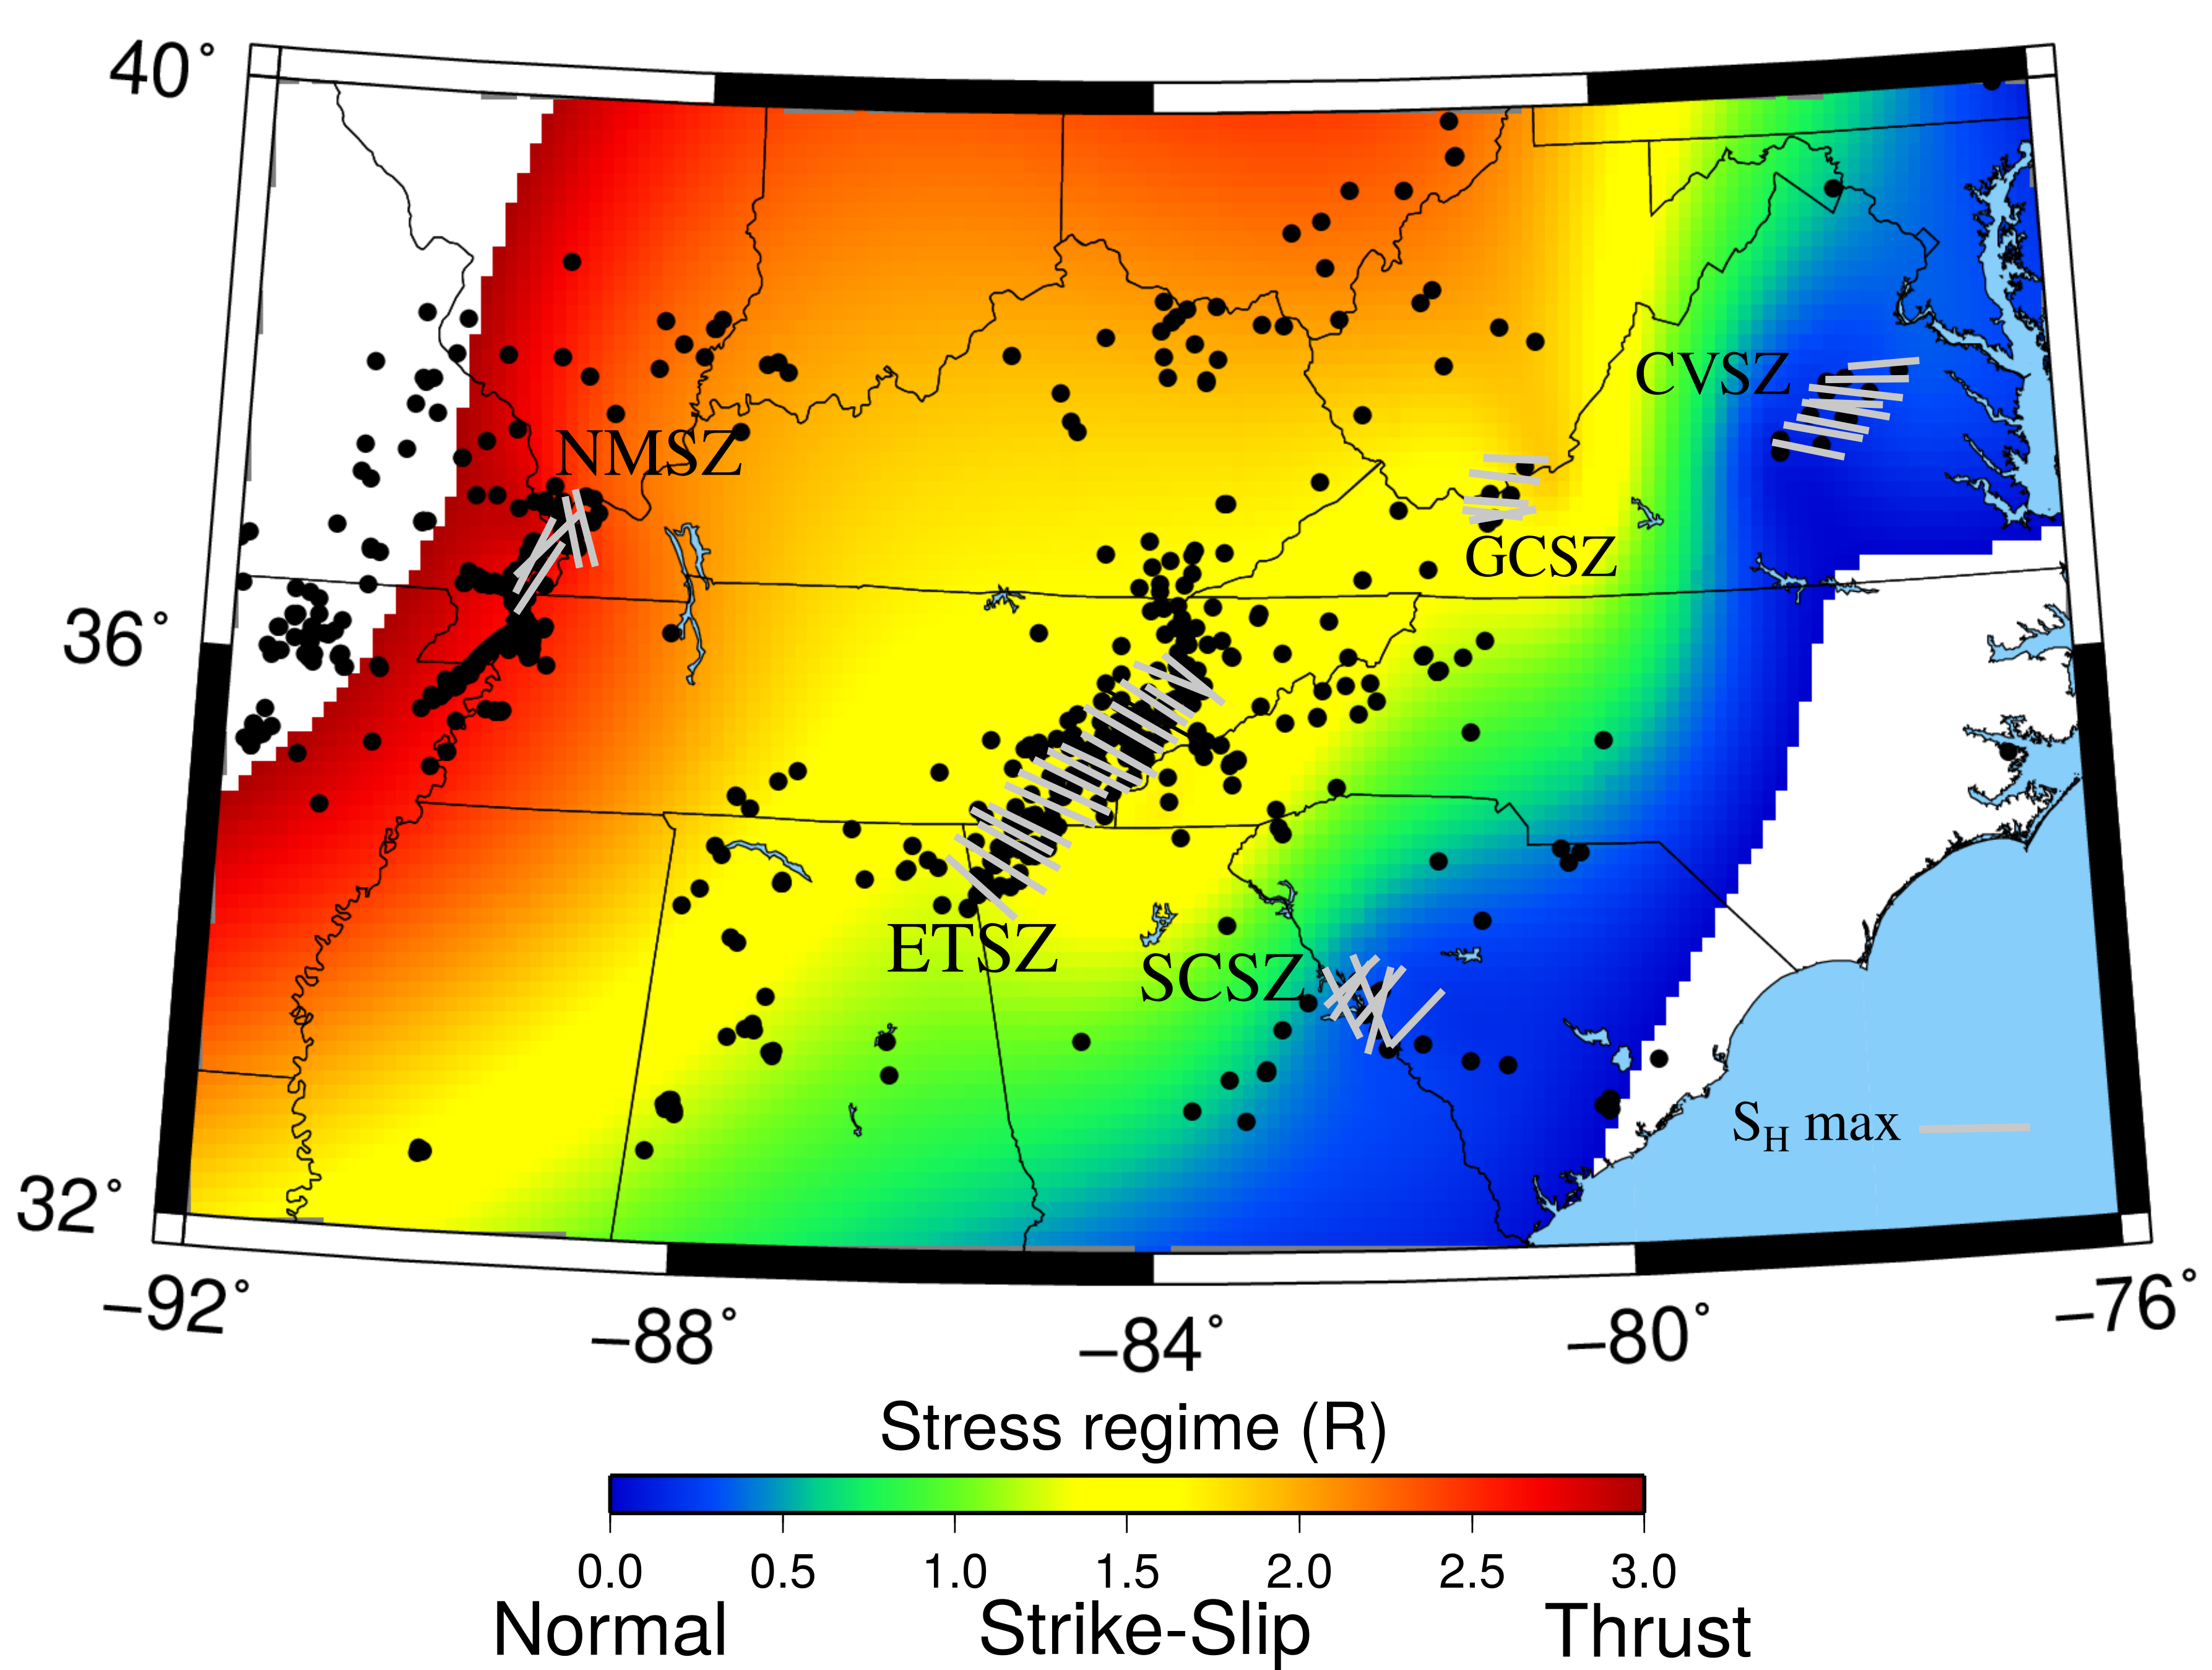
\includegraphics[width=0.75\linewidth]{figures/sigma1.png}
    \caption{Maximum horizontal stress directions (S$_H$) at all the seismic zones for the heterogeneous (HT) model (black lines) overlain over the stress regime (R) computed using the principal stresses at these seismic zones. }
    \label{sigma1}
\end{figure}


    The stresses in our model arise from instantaneous flow due to the upper mantle heterogeneity. Fig. \ref{velocity_pattern} shows the velocity field at slice AA$^{\prime}$ (marked in Fig \ref{fig_model}) in the model HT due to heterogeneous density computed from temperatures based on the tomography study by \citet{Biryol_2016}. A downward velocity flow pattern is found below both the NMSZ and ETSZ and the corresponding upwellings induced by the downward flow are concentrated along the edges of the model domain. The upwellings are observed at the surface as features F$_1$ and F$_2$ marked in Fig.~\ref{df_model}. The downward flow pattern beneath the NMSZ due to the lithospheric drip is opposite to the asthenospheric upwelling proposed by \citet{Biryol_2016}. However, the interpretation of the velocity field from our model depends on various parameters, including the viscosity of the asthenosphere, and boundary conditions of the model. %We computed mantle viscosity solely based on the seismic tomography constraints and the actual value in the earth would be different. 
    Lower viscosity in the asthenosphere would reduce the lateral extent of the convection from the lithospheric drip such that the region surrounding NMSZ is not affected by the downward pull. However, even with lower viscosity asthenosphere, it is still unlikely that the bouyancy effects produced by the localized low-velocity anomaly below the NMSZ (Fig. \ref{fig_tomo}) would counteract the downward pull from the much more significant positive anomaly lithospheric drip. 
    
\begin{figure}[ht]
    \centering
    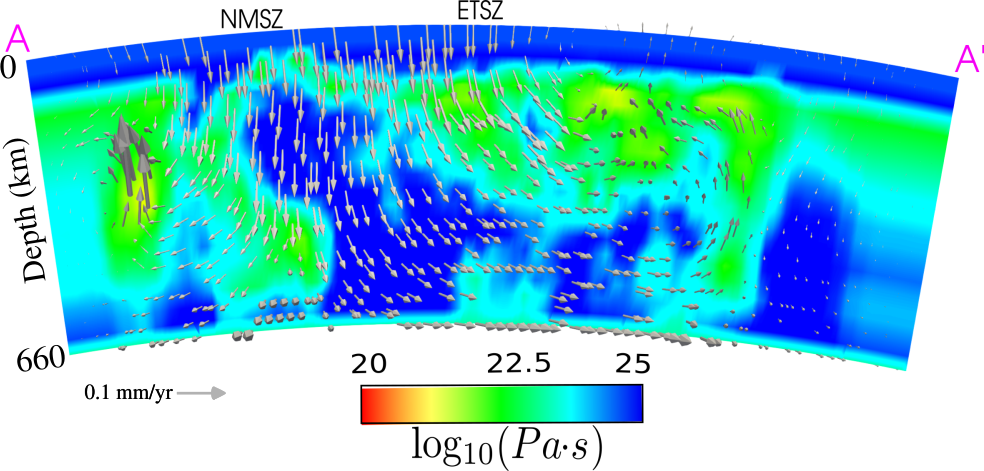
\includegraphics[width=0.9\linewidth]{figures/velocity_pattern.png}
    \caption{Velocity field at slice AA' (marked in Fig \ref{fig_model}) overlying the viscosity distribution computed from the temperatures based on the tomography by \citet{Biryol_2016}. The extreme high-velocity vectors observed west of the NMSZ and out of the plane are from the upward return flow due to the downward pull of the lithospheric drip and are likely an artifact due to fixed boundary conditions at the sides.}
    \label{velocity_pattern}
\end{figure}    
    
%   

\begin{figure}[h!]
    \centering
    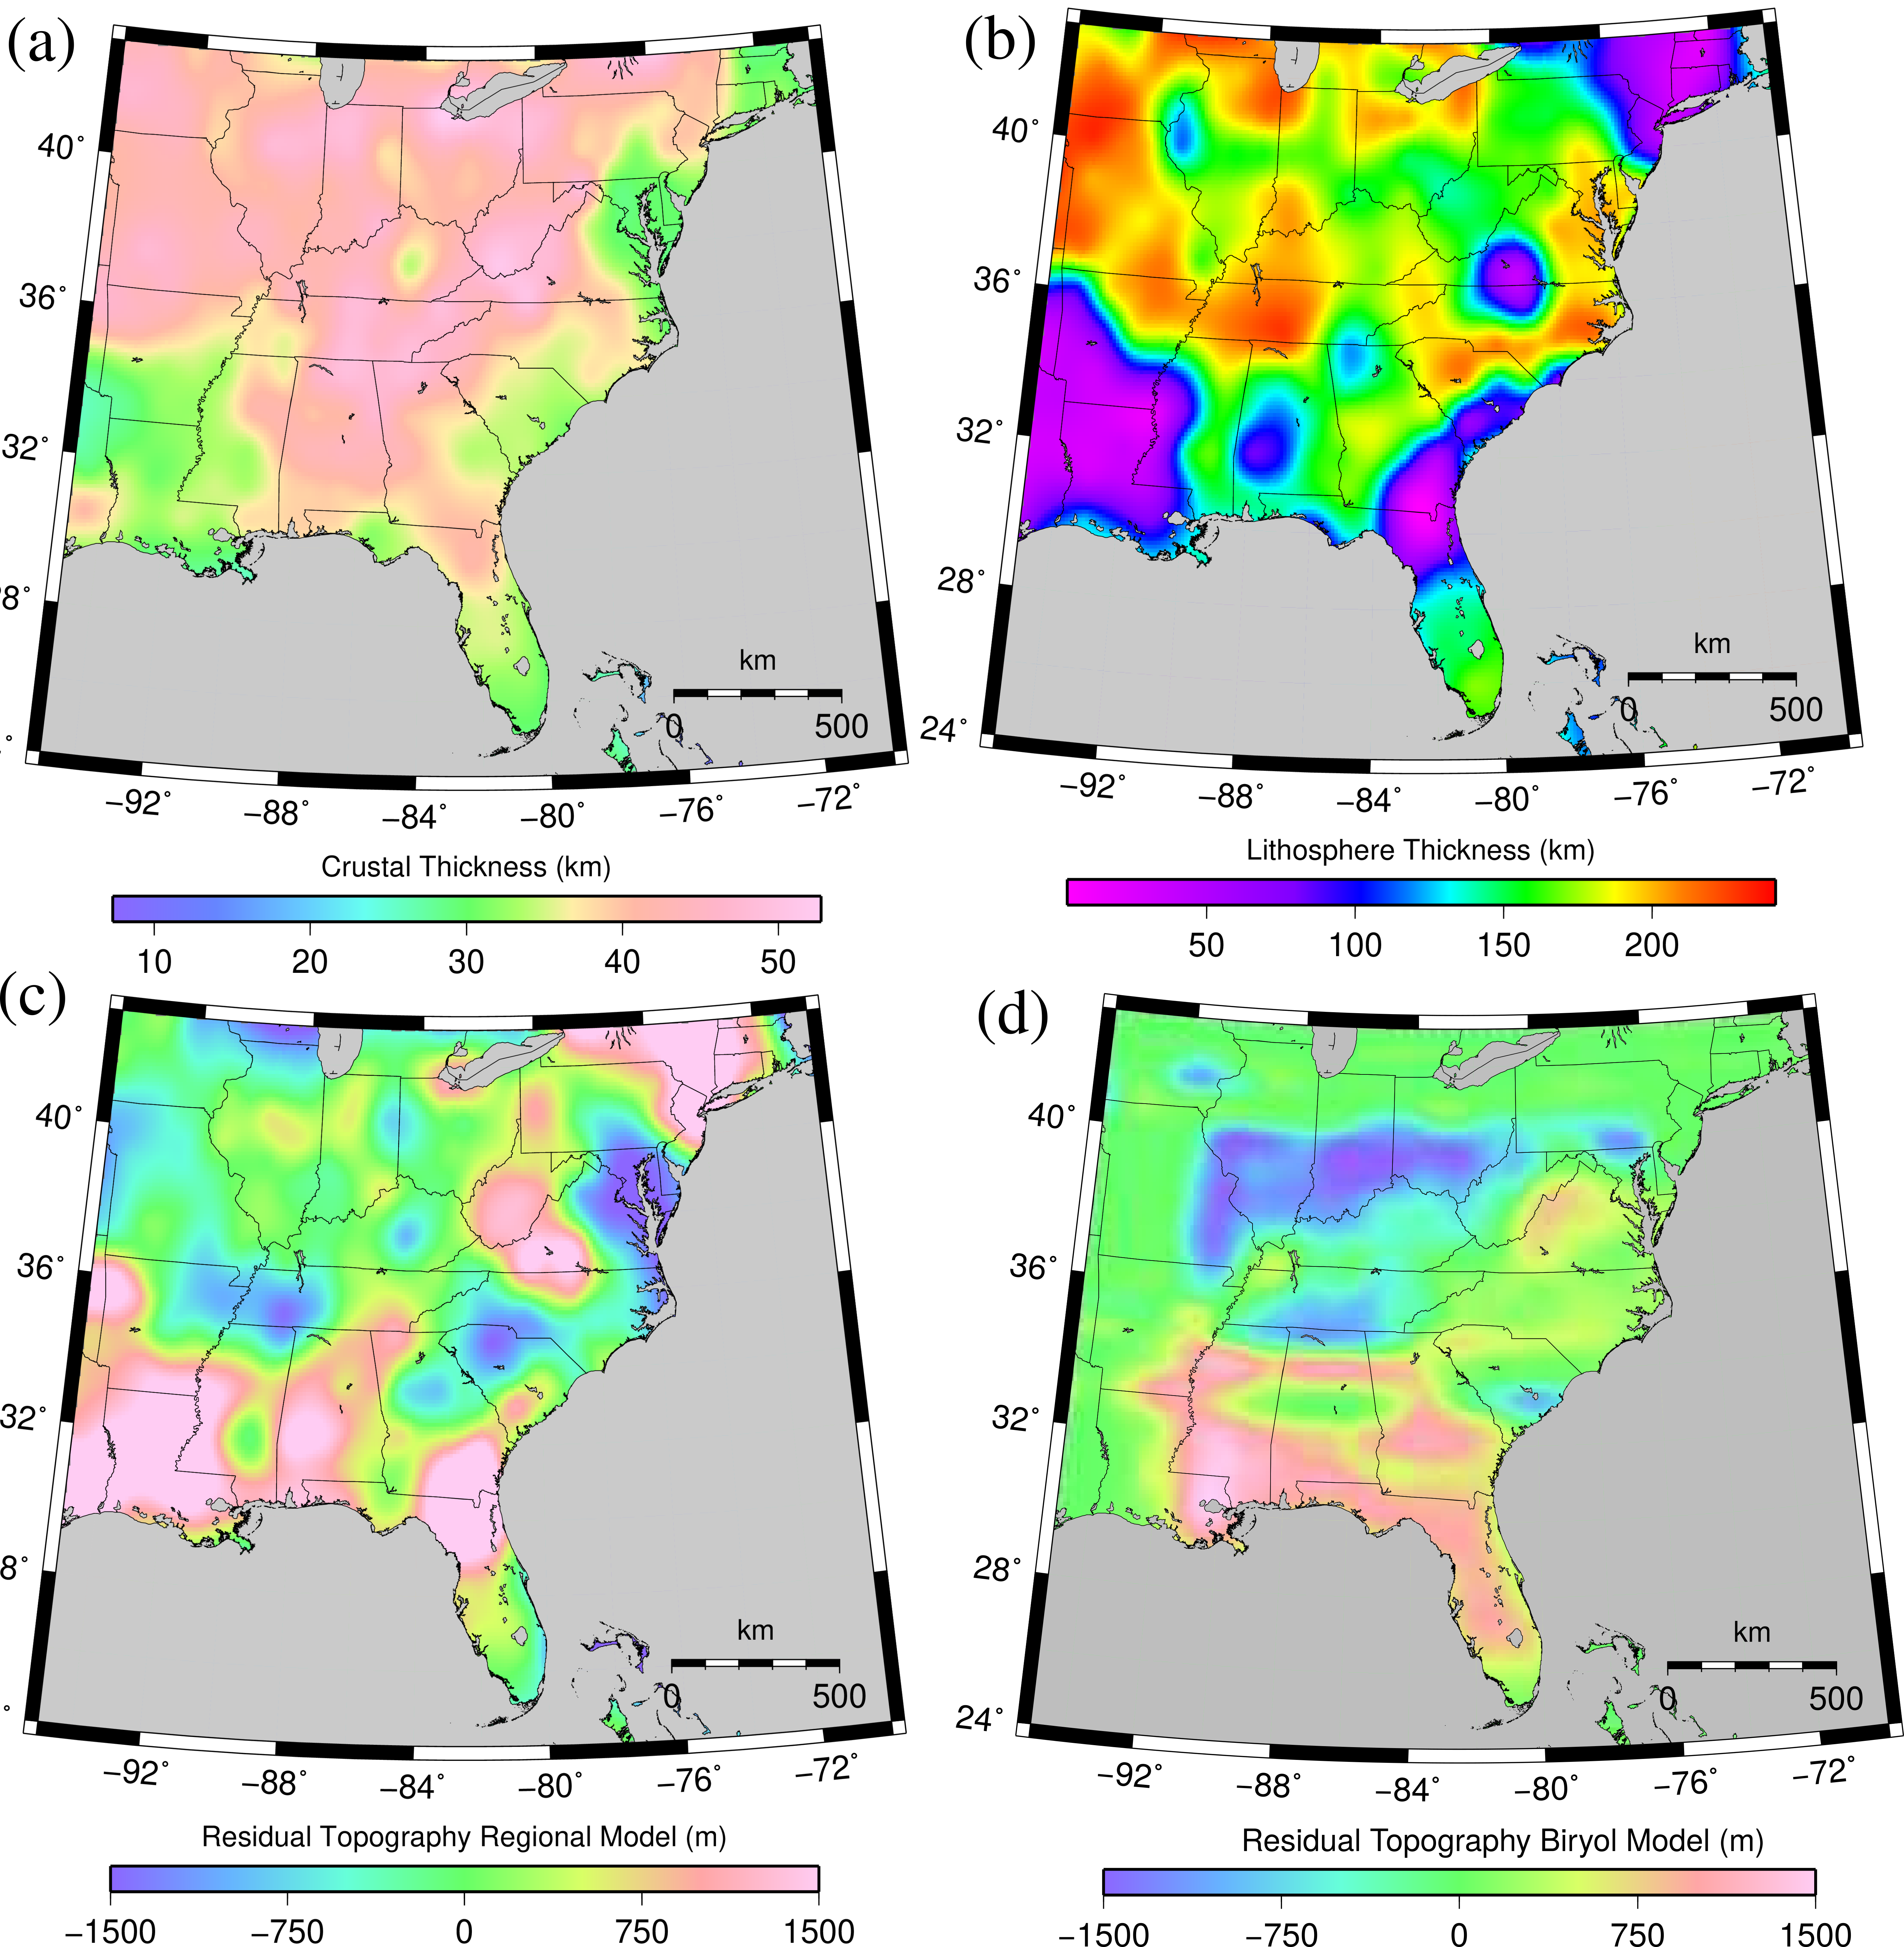
\includegraphics[width=\linewidth]{figures/topography.png}
    \caption{Residual topography calculated from densities based on the regional tomography by~\citet{Biryol_2016} used in this study and from global models. (a) Crustal thickness from CRUST1.0 \citep{laske2013update}. (b) Lithospheric thickness from LITHO1.0~\citep{pasyanos2014litho1} (c) Residual topography calculated using (a) and (b). (d) Residual topography based on the temperatures calculated using the regional tomography used in this study. }
    \label{topo_res}
\end{figure}


% \note[EC]{What is the topographic relief in the study area? It must not be as large as $\pm$2000 m. If so, I'm not sure if it's reasonable that the residual topo has a greater relief than the surface... Maybe but what would be the meaning...?}
    We examined the topography generated due to the mantle flow generated from the upper mantle heterogeneity in Fig. \ref{topo_res}. We calculated residual topography in our study region following the approach by \citet{becker2014static} for the static and dynamic topography for the western US. We first calculate the isostatic topography. We use CRUST1.0~\citep{laske2013update} for crustal thickness and density (Fig. \ref{topo_res} a) and LITHO1.0~\citep{pasyanos2014litho1} for lithospheric thickness variations (Fig. \ref{topo_res}b). We assume a constant lithospheric density of 3300 kg/m$^3$ and a constant asthenosphere density of 3250 kg/m$^3$. These values are reasonable for a density contrast between the lithosphere and asthenosphere~\citep[e.g.,][]{bonnardot2008numerical, ito2011probing}. Although the crustal contribution to the topography is 2.25 times more dominant than the lithosphere for these density values, the residual topography is dominated by the lithospheric variations (Fig. \ref{topo_res}c) which are up to 8 times greater than the crustal thickness variations. We also calculate the residual topography from the mantle flow in our models due to the density distribution based on the \citet{Biryol_2016} tomography results (Fig. \ref{topo_res}d). The discrepancy between the topography calculated using global crustal and lithosphere models and that based on the regional seismic tomography is expected. Firstly, the seismic tomography puts no constraints on the crustal structure, and the crust is assumed to have a uniform thickness of 40 km to calculate the isostatic response, contrary to the crustal thickness and density variations obtained from the CRUST1.0 model. Secondly, the LITHO1.0 model is about eight times coarser in resolution than the tomography study, and we assumed a constant density of 3300 kg/m$^3$ instead of the density based on the heterogeneous temperature. We suggest that continued investigation into accurate crustal and lithospheric thickness and density variations is required to observe any dynamic topography response from the upper mantle flow.
%
    
    We discuss the stress implications of lithospheric foundering using instantaneous models with a drip. Time dependent modeling will be needed to address the mechanism for the origin of a foundering drip in the CEUS. Such an investigation in this region would call for more sophisticated techniques such as backward advection modeling~\citep[e.g.,][]{conrad2003seismic}, quasi-reversibility~\citep{glivsovic2016new}, or adjoint methods~\citep[e.g.,][]{bunge2003mantle, liu2008reconstructing} for the calculation of initial conditions on temperature, viscosity and density, which has not been done in this study. It has been proposed by \cite{Biryol_2016} that the lithospheric foundering could have started due to Rayleigh-Taylor instability beginning from the presence of an ecologized root as proposed by \citet{le2006mantle} in the western US. It is also possible that the dense high velocity mantle feature is part of the subducted Farallon slab below this region~\citep{schmandt2010seismic}. We do not comment on the origin of this high-velocity feature but follow the naming convention by \citet{Biryol_2016} as a drip in this study. Additional observations such as low dynamic topography at the surface would be required to confirm if the high velocity is indeed attached to the lithosphere or is a remnant Farallon slab.
    
    In summary, the numerical model with heterogeneous temperature, density, and viscosity based on the tomography study by \citet{Biryol_2016}, indicates differential stress concentration due to the upper mantle heterogeneity at the major seismic zones in the CEUS: ETSZ, NMSZ, GCSZ, CVSZ, and parts of the SCSZ. We also examine the isolated effect of a positive P-wave velocity anomaly interpreted by \citet{Biryol_2016} as a lithospheric drip and observe increased differential stress in the seismic zones surrounding the root (ETSZ and NMSZ). Coulomb stress was also increased in all the seismic zones at their optimal fault orientations obtained from other studies when all the upper mantle heterogeneity is considered. Therefore, our results provide a possible mechanism for reactivation of the faults in the intraplate seismicity of the CEUS. This, in turn, helps to better associate seismic hazard with the seismic zones in the CEUS.
    
\appendix
\section{Appendix}


\begin{table}
\caption{Mineral physics data used in this study \tnote{1}}
\centering
\begin{tabular}{ l c c c c c c c c c } 
\hline
 \multirow{2}{3em}{Mineral} & \multirow{2}{3em}{Density ($kg/m^3$)} & \multirow{2}{3em}{$K_S$ (GPa)} & \multirow{2}{3em}{$\mu$  (GPa)}  & $K'$ & $\mu'$ &  \multirow{2}{4em}{$\partial K/\partial T$ (GPa/K)}  & \multirow{2}{4em}{$\partial \mu/\partial T$ (GPa/K)} & \multirow{2}{4em}{$a_0 (10^{-4})$} & \multirow{2}{4em}{$a_1 (10^{-7})$} \\ & & & & & & & & & \\
 \hline
  olivine  & 3222 & 129 &  81 & 4.2 & 1.4 & -0.017 & -0.014 & 0.20 &  0.139  \\
  orthopyroxene  & 3215 &  109 &  75 & 7 & 1.6 & -0.027 & -0.012 & 0.387 & 0.044 \\
  garnet  &  3565 & 171 & 92 & 4.4 & 1.4 & -0.019 & -0.01 & 0.099 & 0.116 \\
  wadsleyite  & 3472 & 172 & 121 & 4.5 & 1.5 & -0.014 & -0.014 & 0.232 &  0.0904 \\
  majorite  &  3565  & 171 & 92 & 4.4 & 1.4 & -0.019 & -0.01 &  0.0991 & 0.1165   \\
\hline
\end{tabular}
  \begin{tablenotes}
  \begin {small}
     \item[1] $K_S$: adiabatic bulk modulus, $\mu$: shear modulus, $K'$: pressure derivative of bulk modulus, $\mu'$: pressure derivative of shear modulus, $\partial K/\partial T$: bulk modulus derivative with temperature, $\partial \mu/\partial T$: shear modulus derivative with temperature, $a_0$, $a_1$ are constants in thermal expansivity, $\alpha = a_0 + a_1 T$. Values of elastic moduli and their derivatives are from \citet{Cammarano2003} and thermal expansivity are from \citet{saxena_data}.
     \end{small}
  \end{tablenotes}
 \label{table1}
\end{table}

The effects of composition at high temperature and pressure are incorporated in seismic velocity following \citet{Cammarano2003} in which the elastic moduli ($K$, $G$) and densities ($\rho$) at reference temperature $T_0$ and pressure $P_0$ are first extrapolated at high temperatures ($T$) and then adiabatically at high pressures ($P$) following finite-strain extrapolation \citep{duffy1989seismic}. The calculations are divided at pressures $~$12.5 GPa to account for phase transformation of olivine to $\beta$ spinel at 410 km. 

To calculate density at high pressures, a mantle adiabat with potential temperature ($T_{pot}$) $1300^o C$ was chosen for depths $\leq$ 410 km and $1600^o C $ for deeper depths up to 660 km. Strain ($\epsilon$) is first calculated at known pressures (based on PREM model by \citet{dziewonski1981preliminary}) using $K_0$, $G_0$ and their pressure derivatives, $K_S'$, $G'$  (Table \ref{table1}).  Reference density calculated at the potential temperature and zero pressure ($\rho(T_{pot}, P_0)$) is then used to get the density $\rho (P,T)$.

\begin{align*} 
    P &=  - (1 - 2\epsilon)^{5/2} \left[ 3K_0\, \epsilon + \frac{1}{2} \left( 9K_0 ( 4 - K_S' ) \right) \epsilon^2 \right], \\
    \epsilon &= \frac{1}{2} \left[ 1 - \left( \frac{\rho(T,P)}{\rho(T_{pot}, P_0)} \right) ^{2/3} \right] \\
    \rho(T_{pot}, P_0) &=  \rho(T_0, P_0) \, \exp \left( - \int_{T_0}^{T_{pot}} \alpha (T) dT \right)
\end{align*}
where thermal expansivity, $\alpha(T) = \alpha_0 + \alpha_1 T$ is truncated after the second term. Density changes due to temperature, $T$ from the reference geotherm, $T_o$ and pressure are calculated from above as:

\begin{equation}\label{den_der}
    \delta \rho = \rho(T_0, P_0) \text{exp} \left( - \int_{T_0}^{T} \alpha (T') dT' \right) \alpha(T) ) (T - T_o)
\end{equation}

Temperature dependence on $K$ $G$, is assumed linear while changes in $K_S'$, $G'$ is calculated from the procedure in \citep{duffy1989seismic} as: 

\begin{align*} 
    \delta M\vert_{T, P0} &= \frac{\partial M}{\partial T }  ( T - T_o )\\
    \delta M'\vert_{T, P_0} &=  \left( M'(T_0) \text{exp} \left[ \int_{T_0}^{T} \alpha (T) dT \right] \alpha(T) \right) ( T - T_o )  ,
\end{align*}
where $M$ is either $K$ or $G$, $\delta M$, $\delta M'$ are changes in elastic modulus and its  pressure derviate due to temperature $T$.

Elastic moduli changes are then evaluated at high pressures using second-order extrapolation order expansion \citep{duffy1989seismic}:

\begin{align} \label{M_der}
    \delta K + \frac{4}{3} \delta G &= ( 1 - 2 \epsilon)^{5/2} \left[ M_1 + \epsilon \left( 5 L_1 - 3 \frac{\partial K}{\partial T }  ( T - T_o ) \left[ K' + \frac{4}{3} G' \right] - 3K_0 M_2 \right)  \right], \\ 
    \text{where}, \hspace{0.5cm}
    M_1 &= \delta K\vert_{T, P0} + \frac{4}{3}\delta G\vert_{T, P0} ; \hspace{0.5cm}
    M_2 = \delta K'\vert_{T, P_0} + \frac{4}{3}\delta G'\vert_{T, P_0} \nonumber
\end{align}

The anharmonic velocity variations due to temperature and pressure are then calculated using \ref{den_der}, \ref{M_der} for each mineral and then averaged using Voigt (constant strain) averaging scheme for the reference composition, discontinuous across 410 km,  described in section \ref{temp_var}.

\begin{equation} \label{anh}
    \delta V \vert_{anh} = \frac{1}{2\sqrt{K_0 + 4/3 G_0} \sqrt{\rho_0}} \left[\delta K + \frac{4}{3} \delta G \right] - \frac{K_0 + 4/3 G_0}{1\rho_0^{3/2}} ( \delta \rho)
\end{equation} 

Frequency dependence (anelasticity) of velocity with temperature is incorporated following \citet{Goes_2000}:

\begin{align} \label{anel}
    \delta V \vert_{anel} &= Q_p^{-1} \frac{aH}{2 R T^2 \tan(\pi a/2)},\\
    Q_p^{-1} &= A \omega^{a} \exp \left[ \frac{a(H+PV)}{RT} \right] \frac{3Vp_{0}^{2}}{4Vs_{0}^{2}} \nonumber
\end{align}
Here, $\omega = 2\pi $, values of laboratory constants, $a = 0.15, A = 0.148$, activation energy $H = 500$ kJ/mol, volume $V = 20$ cm$^3$/mol are taken from \citet{sobolev1996upper}. $Vs_0$ and $Vp_0$ are S and P wave velocities from IASP91 \citep{kennett1991traveltimes}.

%We use the equation (\ref{anh}) to calculate anharmonic effects on seismic velocity.
The reference geotherm ($T_0$) for lithospheric (i.e., $<$ 200 km) depths is the one used in~\citep{Goes_2002} for eastern US and for greater depths, we follow Fig. 4.56 from~\citet{turcotte2014geodynamics} due to lack of evidence for regional geotherms at deeper depths. Thermal expansivity ($\alpha$) from~\citet{saxena_data} (see Table~\ref{table1}). We assume a reference composition of harzburgite, i.e., 83 \% olivine (ol), 15 \% orthopyroxene (opx), 2 \% garnet (gt)~\citep{mcdonough1998mineralogy} for depths 40 km to 410 km or pressure (P) $<$ 12.5 GPa. For depths from 410 km to 660 km, we use a reference composition of 60 \% Mg-wadsleyite and 40 \% Majorite~\citep{haggerty1995upper}. We use Burnman, a mineral physics toolbox~\citep{cottaar2014burnman}, to calculate the mantle adiabat with a potential temperature of 1300$^{\circ}$C for P $<$ 12.5 GPa, which is appropriate for continental lithosphere \citep{rudnick1998thermal} and 1600$^{\circ}$ for P $>$ 12.5 GPa~\citep{katsura2010adiabatic}. Values for bulk modulus ($K_S$), shear modulus (G) and density ($\rho$) for each mineral in the composite are taken from~\citet{Cammarano2003} and are listed in Table~\ref{table1}.

%Anelasticity is implemented using~\ref{anel} using the values given by~\citet{sobolev1996upper} 
We account for the anelastic effects on the seismic velocity by correcting for the power law dependence of frequency on seismic attenuation, $Q_p$. We use linear pressure dependence on activation enthalpy ($H(P)= H_0 + VP$, V is the activation volume) in calculating $Q_p$, (model 2 described in\citet{sobolev1996upper}). Another way to correct for pressure dependence on enthalpy is using melting temperature dependence, (model 1 in \citet{sobolev1996upper}, i.e., $H(P)= gRT_m$ where g is constant and $T_m$ is melting temperature). We use model 2 because we do not include the effects of melting in the seismic anomalies for the reasons discussed earlier. We use a value of 1 Hz for the frequency in the attenuation calculation.

The inversion procedure starts with an initial guess for temperature and updates the temperature values at all the observational points in the tomography until the difference of the calculated anomalies with the observed seismic anomalies is minimized. We also calculate temperatures accounting for uncertainties in the elastic moduli and their temperature derivatives as in~\citep{Cammarano2003}) and compare them with the results obtained here using the mean values given in Table \ref{table1}. Taking the maximum values of the elastic parameters reduces the temperature sensitivity such that the negative (positive) velocity anomaly decreases (increases) temperature by a small ($\pm$ 90 K) magnitude. On the other hand, minimum parameter values increase the temperature sensitivity, and therefore the range of temperatures obtained, by $\sim$ 180 K.

Our approach has several differences from that of~\citet{Cammarano2003}. Firstly, we invert velocity anomalies, not absolute velocities, for temperature anomalies, which are added to an assumed reference geotherm $T_o$. Secondly, we use the Voigt averaging scheme to calculate elastic moduli and density of the composite rock instead of the Hashin Shtrikman scheme used by~\citet{Cammarano2003}. Although the Voigt scheme is known to overestimate the converted values~\citep{watt_1976}, seismic velocities based on compositions averaged by the Voigt scheme, which is representative of the upper bound value for the composite~\citep{watt_1976}, and the Reuss scheme, which is representative of the  lower bound value for the composite~\citep{watt_1976}, shows less than 0.2 \% difference in magnitudes. Since this error is within the range of the tomography error \citep{Biryol_2016}, we use the computationally simpler Voigt scheme. Finally, elastic moduli at high pressures are extrapolated using second-order accuracy instead of third-order for simplicity in implementation of the inversion.

%%%

\acknowledgments
We thank Dr. Berk Biryol for sharing his tomography results used for modeling in this study. We also thank the Computational Infrastructure for Geodynamics (geodynamics.org) which is funded by the National Science Foundation under award EAR-0949446 and EAR-1550901 for supporting the development of ASPECT.

%%%%%

%% ------------------------------------------------------------------------ %%
%% References and Citations

%%%%%%%%%%%%%%%%%%%%%%%%%%%%%%%%%%%%%%%%%%%%%%%
% BibTeX is preferred:
%
\bibliography{agusample.bib}
%
% no need to specify bibliographystyle
%%%%%%%%%%%%%%%%%%%%%%%%%%%%%%%%%%%%%%%%%%%%%%%



% Please use ONLY \citet and \citep for reference citations.
% DO NOT use other cite commands (e.g., \cite, \citeyear, \nocite, \citealp, etc.).
%% Example \citet and \citep:
%  ...as shown by \citet{Boug10}, \citet{Buiz07}, \citet{Fra10},
%  \citet{Ghel00}, and \citet{Leit74}.

%  ...as shown by \citep{Boug10}, \citep{Buiz07}, \citep{Fra10},
%  \citep{Ghel00, Leit74}.

%  ...has been shown \citep [e.g.,][]{Boug10,Buiz07,Fra10}.


\end{document}

 Although the stress distribution overlies the seismicity well, our numerical models for the stress computations are only constrained by the temperature conversions from the seismic tomography results by \citet{Biryol_2016} and any errors in the calculated temperature will be transmitted to viscosity and to our stress calculations. 
%
%% ------------------------------------------------------------------------ %%
%
%  IN-TEXT LISTS
%
%% ------------------------------------------------------------------------ %%
%
% Do not use bulleted lists; enumerated lists are okay.
% \begin{enumerate}
% \item
% \item
% \item
% \end{enumerate}
%
